\chapter{Fundamental Concepts}\label{ch:fundamental_concepts}
%%%%%%%%%%%%
%- Short introduction what we will go over.
%%%%%%%%%%%%
This chapter condenses the theoretical concepts that will reoccur throughout this thesis. We start off in Section \ref{sec:xfel} with an introduction to the key aspects of X-ray free electron lasers (XFEL), including the beam operating modes \textit{self-amplified spontaneous emission} (SASE), \textit{self-seeding} and \textit{X-ray pump--X-ray probe}. Section \ref{sec:cluster-theory} is about the formation of rare-gas clusters via supersonic jets and pickup sources. We then dive into the interaction of light and matter in Section \ref{sec:light-matter-interaction} that discusses coherent, elastic X-ray scattering, and inelastic processes in atoms. The chapter ends with Section \ref{sec:ionizatin-of-ext-obj}, describing the nanoplasma formation in pristine cluster and core-shell systems.
%
%
%
\section{Why X-ray free electron lasers?}\label{sec:xfel}
%%%%%%%%%%%%
%- A historic introduction to FELs\\
%%%%%%%%%%%%
%The advance of X-ray free electron laser in the recent years has enabled experimental ideas from long ago but has also opened entirely new branches to research \cite{Pellegrini-2016-RMP,Bostedt-2016-RMP}. So, let us start by investigating how that is. Thus far mostly synchrotron radiation facilities have provided X-rays to a great variety of scientific communities.
%Electromagnetic radiation or light in the X-ray wavelength regime\footnote{Wavelengths of 0.01 of 10nm.} are world famous for their applications in medicine, where X-ray images\index{X-ray!images} allow a non-invasive look inside the body. X-rays are also heavily used in science, where they are heavily used to reveal structures of very small particles, for example proteins - the workhorse bio-molecule in the human body.
X-rays were first created through \textit{Bremsstrahlung}\index{X-ray!Bremsstrahlung}, where an electron beam with kinetic energies $E_{\text{kin}}$ of 100eV - 100keV hit a block of copper and the deceleration of electrons in the copper led to the creation of X-rays. Since then, there has been tremendous progress in the creation of X-rays and they are commonly created in synchrotron facilities for scientific purposes. In a synchrotron facility, electrons are produced in bursts by an \textit{electron gun} and formed to a collimated \textit{electron bunch}. Then, these electrons are accelerated near the speed of light, with kinetic energies, $\gamma$, of $\gamma>\text{ MeV}$, and injected into a storage ring. The electrons are deflected by bending magnets to circle around the ring. The acceleration at the bending magnet leads to the emission of X-rays. Typically, electrons are bunched together to increase the amount of emitted photons and a storage ring can store many electron bunches allowing a high repetition rate of light pulses on the order of megahertz. The X-ray pulses are characterized through a parameter that is called spectral brightness \cite{Mills-2005-IUCR} or sometimes brilliance\index{brilliance|see{spectral brightness}}. We can define the spectral brightness\index{spectral brightness} as \cite{Als-Nielson-2011-JWS}
\begin{equation}
B = \frac{n}{A\ \Theta\ \Delta\! E},
\label{eq:spectral-brightness}
\end{equation}
with $n$ being the number of photons per second, $A$ the source area, $\Theta$ the divergence of the beam, and $\Delta\! E$ being the spectral bandwidth of the light pulse. The spectral brightness is an overall measure of the quality of a light source. The development of modern synchrotron light sources is hence often measured and compared to previously achieved brightness values. The motivation to improve the spectral brightness is manifold and follows the recipe to let a sample interact with as many photons possible, in the shortest time possible, and with the best energy resolution possible. In other words, more brilliant light sources enable imaging of even smaller particles, or investigate dynamics that are even faster.\\[1\baselineskip]
\begin{figure}[t]
	\centering
		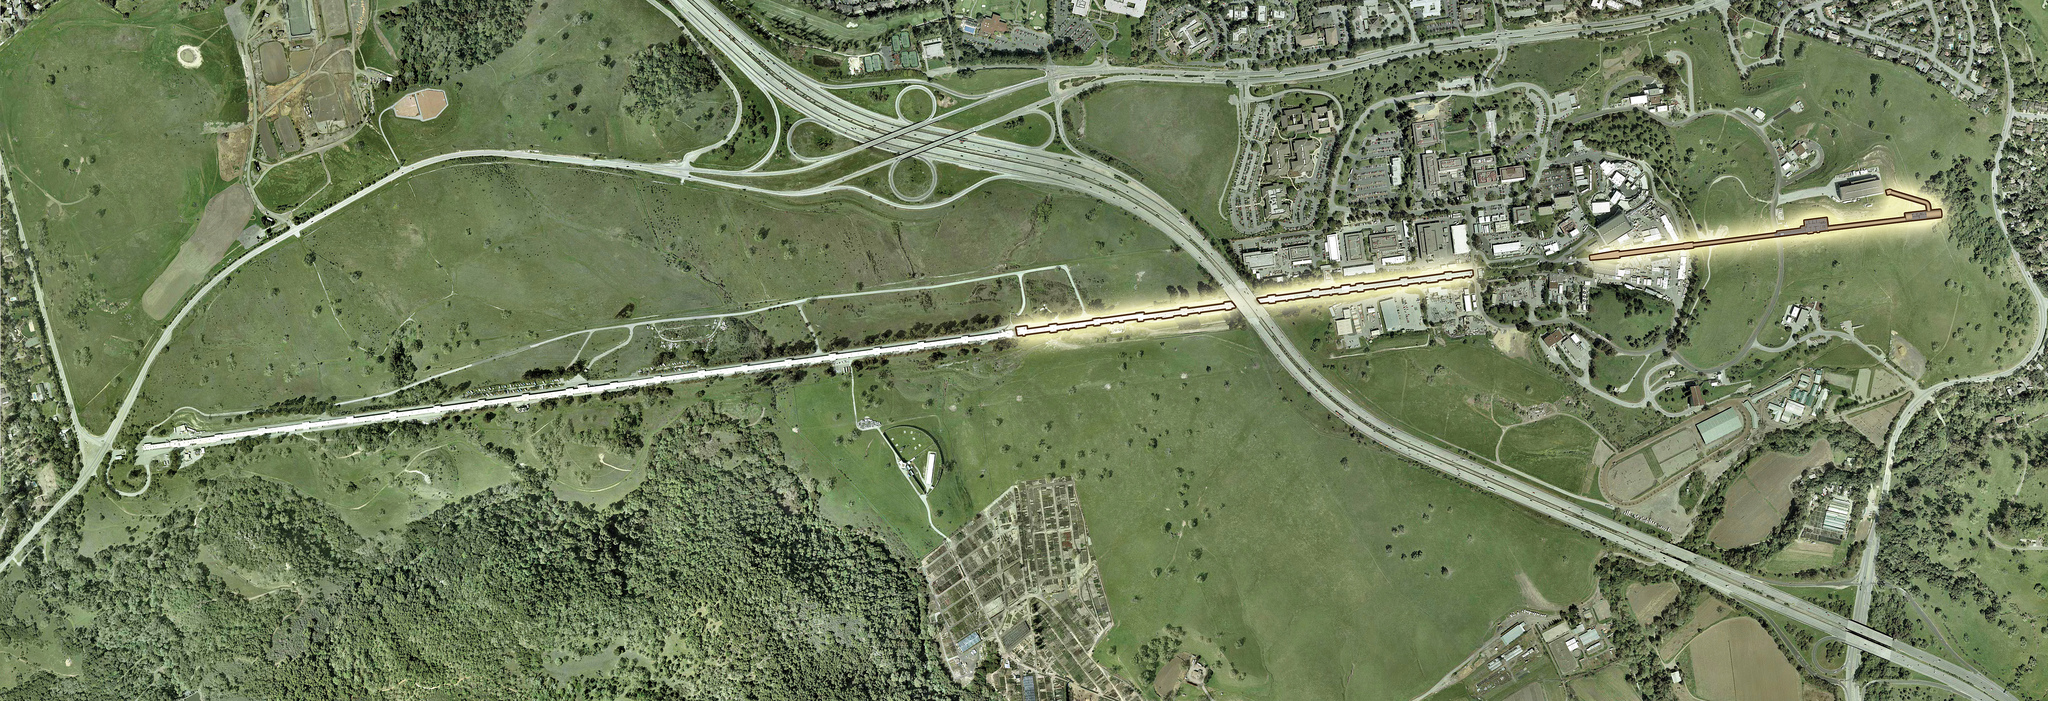
\includegraphics[width=1.00\textwidth]{images/aerial-view-lcls.jpg}
	\caption[Aerial view of the Linac Coherent Light Source.]{Aerial view of the Linac Coherent Light Source\index{Linac Coherent Light Source} (LCLS). LCLS\index{LCLS|seealso {Linac Coherent Light Source}} uses the last third of the SLAC Linear Accelerator but is overall a $\sim 4.1$ km long machine. The accelerator and buildings are stretched far because of the light generation process. From \cite{SLAC-2009-Flickr}}
	\label{fig:aerial-view-lcls}
\end{figure}
To get a numerical understanding, let us look at non-linear absorption dynamics in atoms and molecules. One can conservatively estimate that a typical absorption cross section at soft X-rays\footnote{Soft X-rays have wavelengths of 10 nm to $\sim 0.2$ nm.} is around $\sigma = 1$ megabarn (Mb) \cite{Bucksbaum-2011-Book}. Typical X-ray focii\footnote{The focus size at the AMO instrument of LCLS is $\SI{1}{\micro\meter\squared}$.} are $A = \SI{1}{\micro\meter\squared}$ such that the number of photons, $n_{in}$, needed to absorb just one photon per atom, $n_{abs}$, is
\begin{equation}
n_{in} = \frac{n_{abs} A}{\sigma} = \frac{10^{-8} \mathrm{cm}^{2}}{10^{-18} \mathrm{cm}^{2}}=10^{10}\qquad \mathrm{photons.}
\label{eq:absorption-cross-section}
\end{equation}
We can compare this to a modern synchrotron source, e.g., NSLS-II. This synchrotron produces $1.7 10^{4}$ photons per pulse in the Si(111) bandwidth at pulse durations of a few tens of picoseconds \cite{Williams-2016-PC}. That is far out of reach for investigating non-linear, or multi-photon, processes. While this back of the envelope type of calculation might be off by an order of magnitude or so depending on the specific case, it illustrates the order of magnitude improvement scientists were looking for to unravel entirely new aspects of nature. As it is not possible to use conventional optical methods to increase the number of X-ray photons there were drastic ideas. A progressive United States defense program in the 80's ignited an atomic bomb to create an X-ray beam that was intended for use as anti-(space)missile defense \cite{Hecht-2008-OPN}. In a similar time, it was also proposed to build free electron laser \cite{Kondratenko-1980-PA,Bonifacio-1984-OC} to increase the spectral brightness.\\[1\baselineskip]
%
Free electron lasers, amplify the light along a straight line to create optical laser-like radiation. Construction of the first hard XFEL finished in 2009 and it is called the Linac Coherent Light Source\index{Linac Coherent Light Source}. LCLS can be seen from a birds-eye view in Figure \ref{fig:aerial-view-lcls}. XFEL are able to create $10^{12}$ photons per pulse and achieve pulse lengths of a few femtoseconds. The beam parameters of the XFEL increased the spectral brightness of user facilities by many orders of magnitude\footnote{See Figure \ref{fig:soft-xray-self-seeding} for an illustration of the improvement in brilliance.}. This allows the study of, for example, the ultrafast movement of electrons in chemical reactions \citep{Dell'Angela-2013-Science,Picon-2016-NatComm}, the imaging of nanoparticles \citep{Chapman-2011-Nature,Seibert-2011-Nature} and the discussed nonlinear dynamics of atoms, molecules and clusters \citep{Young-2010-Nature,Rohringer-2012-Nature,Berrah-2011-PNAS,Gorkhover-2012-PRL}.\\[1\baselineskip]
%
Only a few XFEL exist today. The LCLS at SLAC National Accelerator Laboratory (SLAC) in the United States and the SACLA at Rikagaku Kenkyūsho (RIKEN) in Japan are the two currently operating XFEL user-facilities. Due to their success, more XFEL are being built around the world, for example, the European XFEL near Deutsches Elektron Synchrotron (DESY) in Germany, the SwissFEL at Paul Scherrer Institut (PSI) in Switzerland, and the PAL-XFEL at Pohang Accelerator Laboratory (PAL) in South Korea.
%
%
%
\subsection{From bending magnets to undulators}\label{sec:undulator}
%%%%%%%%%
%- Idea and schematic setup\\
%- Explain SASE including micro-bunching\\
%- Talk about the importance of monitoring the energy loss
%%%%%%%%%
\begin{figure}[t]
	\centering
		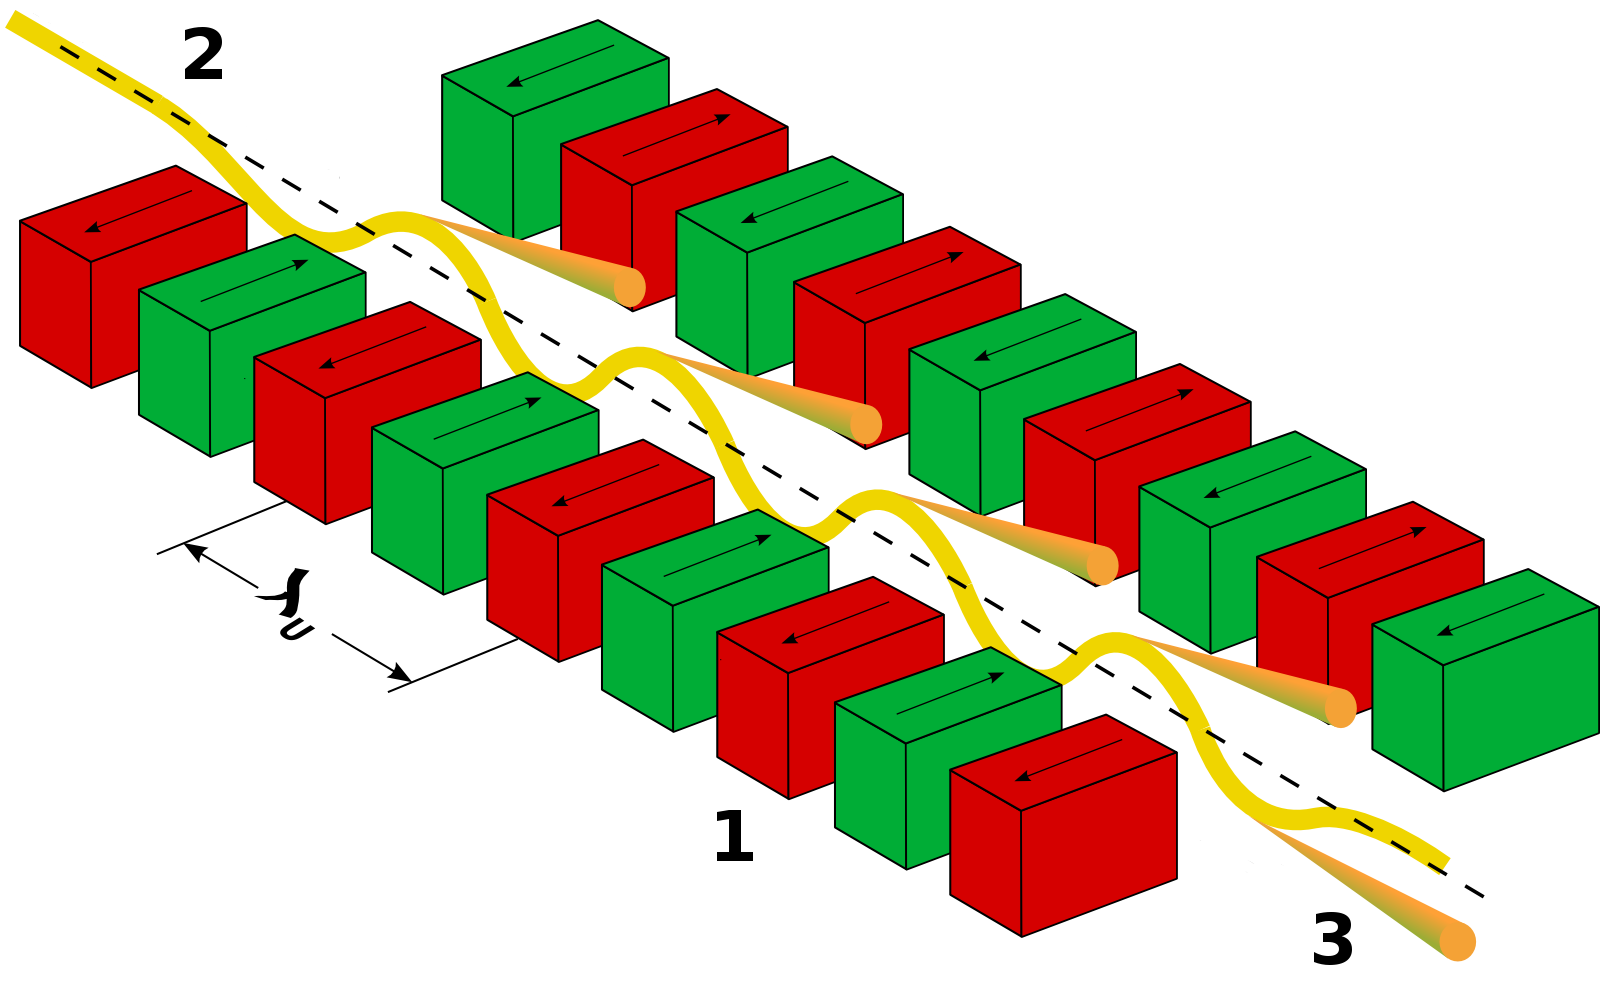
\includegraphics[width=1.00\textwidth]{images/Undulator.png}
	\caption[Schematic setup of an undulator.]{Schematic setup of an undulator with a period of $\lambda_{U}$. (1) Magnets in alternating polarity; the arrows indicate the direction of the magnetic field. (2) Incoming electron bunch near the speed of light. (3) Emitted light in beam direction due to sinusodial movement of the electron bunch. From \cite{holst-2005-wiki}.}
	\label{fig:undulator}
\end{figure}
In the beginning of X-ray lightsources\index{lightsource}, the radiation was generated using \textit{bending magnets}\index{bending magnets}. A bunch of electrons was accelerated near the speed of light and traversed a bending magnet. The acceleration from the magnet resulted in the emission of electro-magnetic radiation. The first improvement to creating X-rays over bending magnet sources was through a \textit{wiggler}\index{wiggler}. Wigglers consist of magnets arranged in an alternating order. An electron bunch traveling through a wiggler is ``wiggled'' along its path due to magnetic fields, which causes the particles to emit radiation. Wigglers can be considered as a series of bending magnets, which is why the total emitted power, $P_{emitted}$, is proportional to the number of magnets, $m$, \citep{Brown-1983-NIMPR}
\begin{equation}
P_{emitted} \propto m,\quad \text{in a wiggler magnet.}
\end{equation}
The emitted radiation has a broad, continuous spectrum and the center of that spectrum can be controlled by changing the speed, or kinetic energy, of the electron bunch. Wigglers were used at the Stanford Synchrotron Radiation Lightsource (SSRL) in 1979 to generate X-rays. Independently from wigglers, undulators\index{undulator} were developed \citep{Williams-2009-xb}. A schematic setup of an undulator can be seen in Figure \ref{fig:undulator}. Wigglers and undulators create radiation on the same principle: an electron bunch is accelerated near the speed of light and then forced on a sinusoidal pathway. In undulators, the separation of magnets is specific and named undulator period, $\lambda_{U}$. The undulator period and magnetic fields are chosen such that their emitted radiation per period constructively interfere with each other. Thus the emitted power, $P_{W}$, now scales as \citep{Kim-1986-NIMPRA}
\begin{equation}
P_{\text{emitted}}\propto m^{2},\quad \text{in an undulator magnet.}
\end{equation}
The X-rays emitted by undulators have typically a narrower spectrum and a higher flux than wigglers. We can further characterize undulators (and wigglers) by the strength parameter, $K$, which is given by, \citep{Huang-2007-PRSTAB}
\begin{align}
K &= \frac{e\ B_{\text{max}}\ \lambda_{U}}{2 \pi\ m_{e}\ c},
\intertext{with $e$ being the elementary charge, $B_{\text{max}}$ being the maximum magnetic field in the undulator (wiggler), $m_{e}$ being the mass of an electron and $c$ being the speed of light, we can write in convenient units}
K &\approx 0.934 B_{max}\ \lambda_{U}\qquad \left[\mathrm{T\ cm}\right].
\label{eqn:undulator-strength}
\end{align}
Undulators typically have $K < 1$ Tcm (and wiggler $K\gg1$ Tcm). Undulator magnets are large constructs of a few meters and their undulator period is on the order of centimeters. The electrons emit radiation in the nanometer wavelength regime because electrons near the speed of light have to be considered relativistic. In the frame of the electrons, the undulator period, $\lambda_{U}$, appears shorter. We can account for the relativistic effects and express the resonantly amplified wavelength, $\lambda_{r}$, by \citep{Huang-2007-PRSTAB}
\begin{equation}
\lambda_{r} = \frac{\lambda_{U}}{2 \gamma}\left(1+\frac{K^{2}}{2}+\gamma^{2}\Psi^{2}\right),\label{eqn:fundamental-wavelength}
\end{equation}
with the kinetic energy $\gamma$ of the electron bunch in the undulator and the electron observation angle $\Psi$.\\
%Summarizing, modern lightsources use undulators to generate radiation as these magnets create more photons that have a narrow spectral bandwidth compared to bending magnets and wiggler. Undulators are characterized by the strength parameter given in Equation \eqref{eqn:undulator-strength}, which is only dependent on the undulator gap $\lambda_{U}$ and the magnetic field $B$. The fundamental amplified wavelength is given by the resonance condition Equation \eqref{eqn:fundamental-wavelength}.\\
\begin{figure}
	\centering
		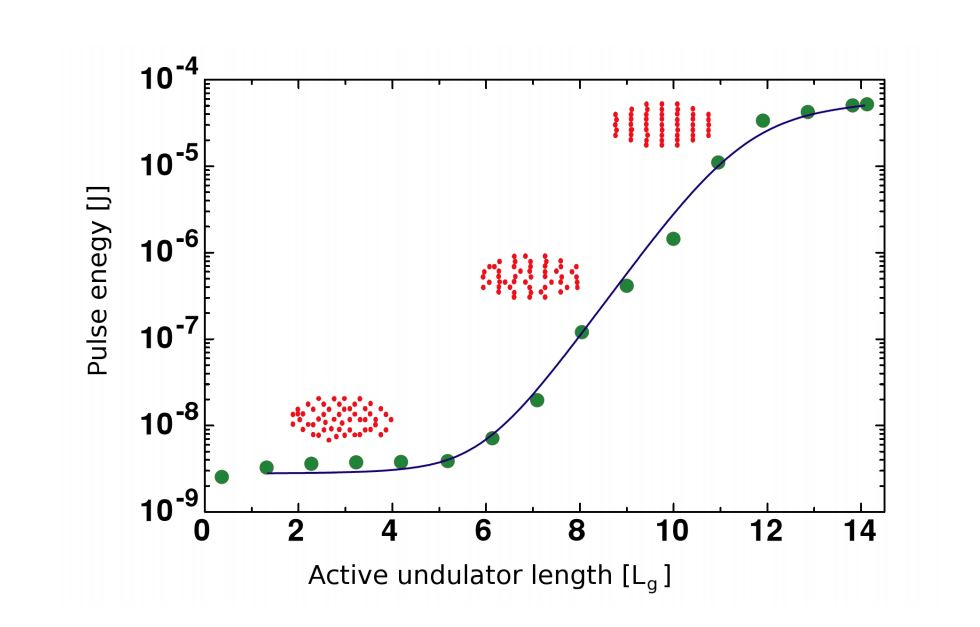
\includegraphics[width=0.75\textwidth]{images/gain-length.JPG}
	\caption[Undulator gain curve correlated to microbunching.]{Undulator gain curve correlated to microbunching. The X-ray pulse energy is plotted logarithmically over the undulator length $L_{g}$ (blue curve, green dots) and shows an exponential growth until saturation. The electron bunch (red dots) starts with a random density distribution. As the bunch travels through the undulator, its density is modulated periodically such that the electrons microbunch. Upon optimal \textit{microbunching}, the X-ray lasing process saturates. From \citep{Rupp-2013-Thesis,Rupp-2016-Springer}}
	\label{fig:gain-length}
\end{figure}
\subsection{Self-amplification by spontaneous emission}\label{sec:sase}
If an electron bunch travels through just one undulator, the emitted power scales linearly with the number of electrons, $N_{e}$, which is due to the finite size and randomly distributed density of an electron bunch. If the electrons emit light from the same point or separated by $n\ \lambda_{r}$, with $n=\left(1, 2, 3, ...\right)$, the emitted photons would constructively interfere. XFELs use this idea to generate their light pulses. XFELs have a straight and long undulator section\footnote{LCLS has a 112 m long undulator section.}, where multiple undulators are connected in series. As the electron bunch travels through the XFEL undulator section, microscopic effects play a role that could be neglected in typical synchrotron radiation sources. In vacuum, light will always be faster than electrons. This slight velocity difference means that the co-propagating photons and electrons have a phase difference and interact with each other. Depending on the phase, an electron will either gain or lose velocity. Over each undulator period, we can describe this \textit{slippage}\index{slippage} with $\lambda_{r}(\Psi = 0)$. As a result, the initial uniform electron density is periodically modulated as it travels through the undulators of a FEL. The modulated electron bunch structure is called \textit{microbunching}\index{microbunching}. The increasingly structured electron beam amplifies a narrower wavelength bandwidth and the number of electrons that are in phase with the photons increases over the travel length through the undulator. The lasing process saturates when the microbunching is fully developed. This process is illustrated in Figure \ref{fig:gain-length}.
The microbunching is defined by the initially emitted photons of pseudo-random wavelength, since the bunch amplifies these specific wavelengths as it travels through the undulators through subsequent spontaneous emission.
%Initially (random) created photons in the undulator define the microbunching as it travels through the undulators and amplifies these photons through subsequent spontaneous emission. 
Hence, this type of radiation (or XFEL operation mode) is called \textit{Self-Amplification by Spontaneous Emission} (SASE). SASE achieves laser-like amplification of the radiation power $P_{SASE}$ scales as \citep[see][p.~61]{Als-Nielson-2011-JWS}
\begin{equation}
P_{SASE} \propto N_{e}^{2},\quad \text{SASE operation.}
\end{equation}
SASE spectra can be seen in Figure \ref{fig:SASE-spectra}. A SASE spectrum is different from shot-to-shot and has distinct peaks that are defined by the initial photons on top of a more broad background.
\begin{figure}
	\centering
		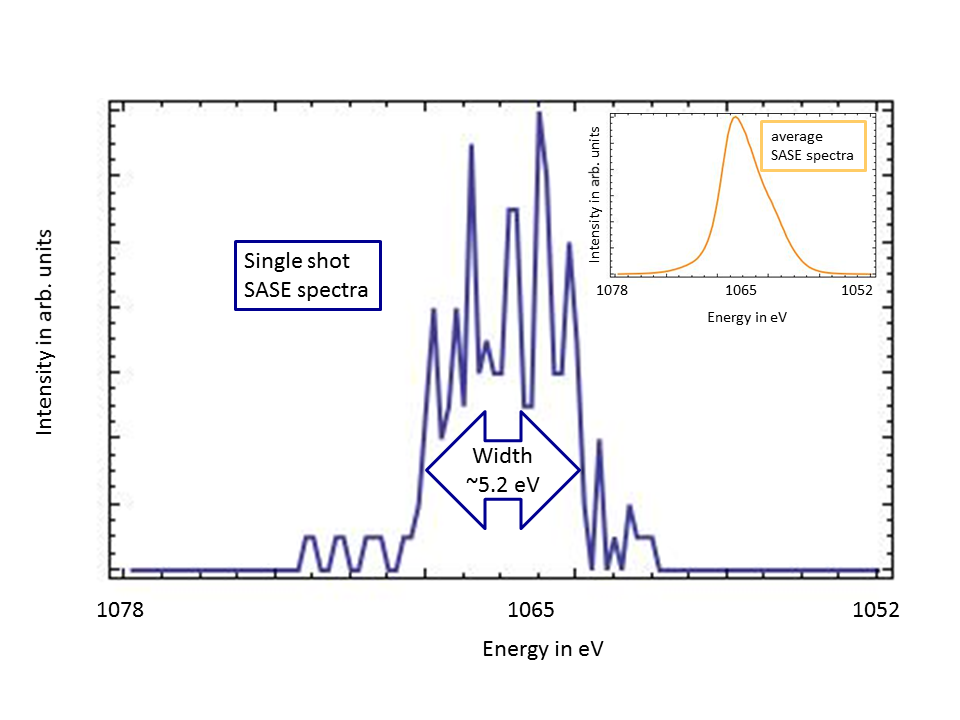
\includegraphics[width=0.60\textwidth]{images/SASE-spectra.png}
	\caption[SASE single-shot and average spectra]{The large blue spectra is a SASE spectra from a single LCLS shot measured with a photoelectron \citep[see][]{Bucher-2014-Unpublished}. Note the spiky peak structure on a background pedestal. Within the narrow bandwidth of an XFEL pulse some energies are more strongly amplified due to the microbunching. The yellow graph in the inset is an average spectrum of several hundred single-shots and shows a low energy tail, which is due to XFEL-jitter.}
	\label{fig:SASE-spectra}
\end{figure}
The electrons interact with the photon-field because of the narrow spatial and kinetic energy distributions that define the so-called \textit{emittance}\index{emittance} of an electron bunch. Only the linear accelerator components of an FEL are able to compress an electron bunch in space and energy, i.e., create a low emittance electron bunch, such that it can interact with the photons and microbunch. Since the creation of X-rays affects the kinetic energy of the electron bunch, $\gamma$, and the lack of optics, XFELs use one (compressed) electron bunch\footnote{the European XFEL uses a so-called \textit{bunch train}, where multiple electron bunches are accelerated in series.} in a long set of undulators to create one light pulse. This is also called a \textit{single-pass high-gain} FEL. Without going into much detail, optics can be used to build \textit{multi-pass low-gain} FEL that are able to reuse electron bunches \citep{Kim-2008-PRL}, which leads to higher repetition rates and more narrow spectrum but fewer photons per pulse.
%
%
%
%
\subsection{Soft X-ray self-seeding}
%%%%%%%%%%%%%%%%%%%%%%
%- Should I include this section? I could use it for the pump probe as well\\
%- Self seeding vs. seeded FELs\\
%- Schematic setup of a self seeding unit\\
%- Work towards self-seeded beams including spectrometer data
%%%%%%%%%%%%%%%%%%%%%%
\begin{figure}
	\centering
		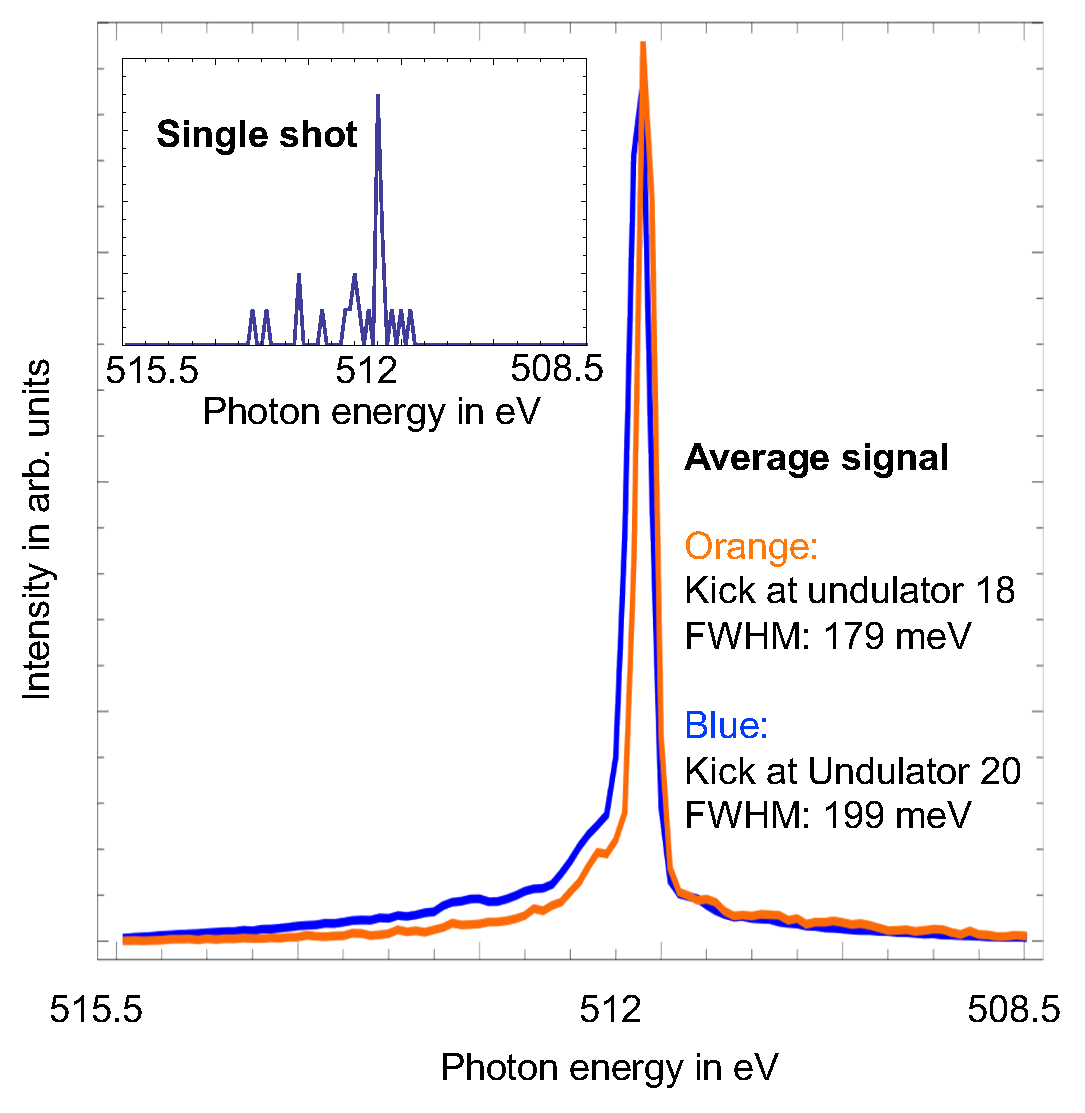
\includegraphics[width=0.49\textwidth]{images/Soft-X-ray-self-seeding.pdf}
		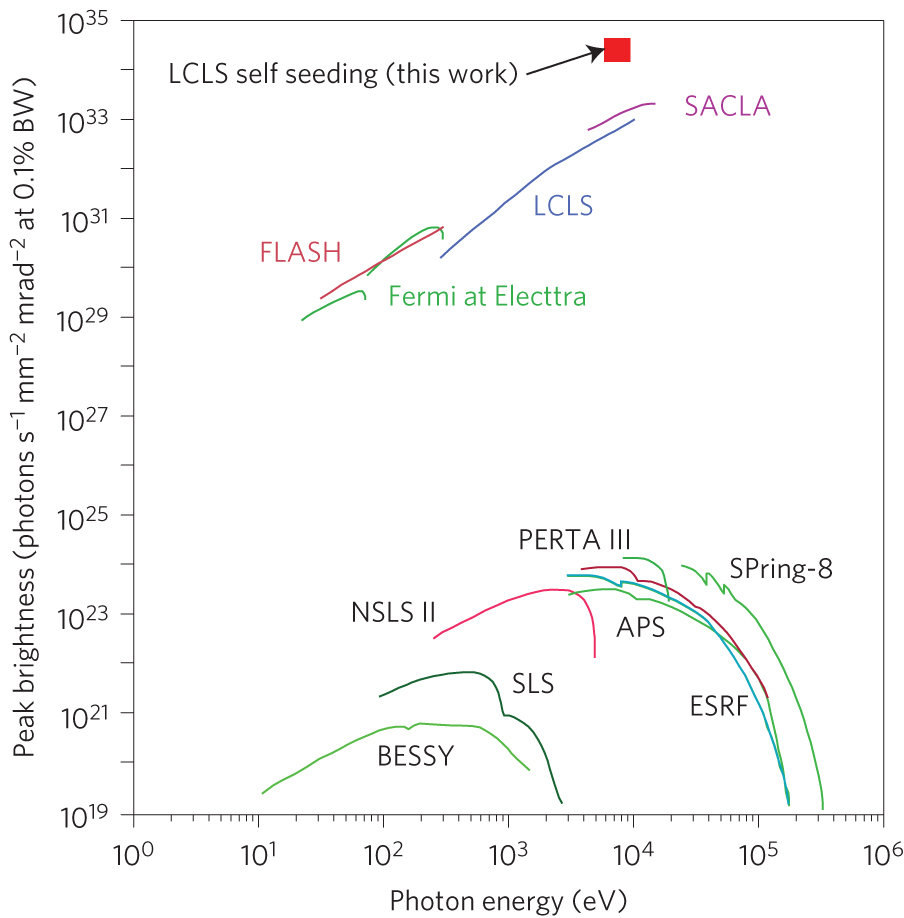
\includegraphics[width=0.49\textwidth]{images/spectral-brightness-fletcher-2015.jpg}
	\caption[Soft X-ray self-seeding spectra and brilliance of various lightsources.]{Left, normalized average spectra of soft X-ray self-seeding (SXRSS) operations using the AMO instrument at LCLS \cite[see][]{Bucher-2014-Unpublished}. The self-seeding spectra is characterized by a sharp spectral peak around a desired energy accompanied by a SASE-radiation-type spectral pedestal. The often undesired SASE pedestal is suppressed, when the electron bunch travel through undulators is shortened. The right image shows the peak spectral brightness of various light sources over a wide photon energy range. SXRSS operations have a spectral brightness that exceeds current SASE FEL sources. From \citep{Fletcher-2015-NatPho}.}
	\label{fig:soft-xray-self-seeding}
\end{figure}
Another free electron laser (FEL) beam mode is the seeded type. In contrast to the SASE operation, where the initial photons are randomly emitted and further amplified, a seeded FEL starts with a given \textit{seed} of photons. If the set of initial photons is monochromatic, mostly this wavelength is amplified as the bunch travels through the undulator along-side the seed. The initial photon seed can be created through various processes and the wavelength of the photon seed is the critical parameter in determining which method to choose. For example, in the case of the infra-red (IR) to extreme ultra-violet (XUV) wavelength range, conventional lasers can be used to produce the initial photon seed. However, due to the lack of lasers available at X-ray wavelengths, the idea of \textit{self-seeding}\index{self-seeding} gained traction. In self-seeding, an electron bunch is first sent through a few undulator magnets to generate a few SASE photons, the electrons and photons are then separated using a magnetic chicane, which also neutralizes the microbunching in the electron bunch. The monochromator selects a small wavelength slice from the comparably broad SASE spectrum of the initial photons. Photons exiting the monochromator are considered as \textit{seed}. The seed and the electron bunch are overlapped again using the magnetic chicane and then sent through more undulators. Here, the seed modulates the electron bunch and thus only a narrow spectral band is amplified. A typical spectrum of a soft X-ray self-seeded beam can be seen in the left panel of Figure \ref{fig:soft-xray-self-seeding}. The characteristics of a self-seeded spectrum are an intense peak at the selected wavelength regime on top of a broad SASE background pedestal. The background is an artifact of the amplification of some spontaneous emission events and can be suppressed by using fewer undulator magnets. Self-seeded beams have a significantly reduced pulse energy -- by an order of magnitude, depending on the exact beam parameters -- as compared to LCLS SASE operations. However, in their main peak, self-seeded beams have a higher spectral brightness when compared to a SASE beam. Using Equation \eqref{eq:spectral-brightness}, the increase in spectral brightness compared to SASE is understandable and it is illustrated in the right panel of Figure \ref{fig:soft-xray-self-seeding}. Self-seeded beam operations have recently been demonstrated at LCLS. For hard X-rays, the Hard X-Ray Self-Seeding (HXRSS) instrument uses a diamond crystal to select a wavelength slice \citep{Amann-2012-NatPho}. At soft X-rays, the Soft X-ray Self Seeding (SXRSS)\index{self-seeding!soft x-ray} instrument uses a grating in a dispersive monochromator \citep{Ratner-2015-PRL}. A seeded beam using an external laser to generate photons as an initial seed has been demonstrated at the XUV-FEL FERMI at Ellettra-Sincrotrone (ELETTRA) in Italy \citep{Allaria-2012-NatPho}. The peak intensity in a narrow spectral band makes seeded beams interesting for a variety of applications, particularly in spectroscopy, where it is instrumental to excite materials with narrow bandwidth photons. There are also applications in atomic and molecular physics, ranging from linear absorption spectroscopy \citep{Ferguson-2014-Unpublished}, to ultrafast photoemission spectroscopy on molecules \citep{Bucher-2014-Unpublished}, to non-linear stimulated Raman spectroscopy \citep{Kimberg-2016-FD}, to ultra-fast photoemission studies. Particularly interesting for this work is the magnetic chicane from the SXRSS instrument when used as described in the next chapter.
%
%
%
%
\subsection{Novel X-ray pump–X-ray probe techniques}\label{sec:novel-pump--probe-tech}
%%%%%%%%%%%%%%%%%
%- Albertos pump-probe version\\
%- Agos two color pump probe version\\
%- Ratners and Agos seeded pump probe version\\
%- Use spectra from single-shot spectrometer
%%%%%%%%%%%%%%%%%%%%%%%%
In order to study X-ray induced phenomena using X-ray imaging and spectroscopy techniques, as it is discussed in this thesis, two X-ray pulses are needed. Here, a pump-pulse is used to induce dynamics in the sample system and a probe-pulse is used to probe them at a certain time delay. Pump--probe experiments are commonly used as they allow a precise study of dynamics. The pump-pulse gives a very controllable starting point, i.e., ``time zero'' in the dynamic process, and the probe-pulse can perform a measurement at a later time delay, $\Delta t$. Sometimes pump- and probe-pulse are switched, which is indicated by a negative time delay to verify time zero, or to probe the system before any dynamics have occurred. It is often desirable to have a pump- and probe-pulse of different wavelength. XFEL can produce two X-ray pulses of different wavelength and such types of operation are called ``two-color'' pump--probe schemes, which we will discuss in the following.\\[1\baselineskip]
%
Creating two X-ray flashes to conduct a pump--probe experiment is a technical challenge, again, due to the lack of efficient X-ray optics. In order to overcome this challenge, two methods have been proposed. Method one is a mirror based beam-split and delay system \citep{Castagna-2013-JPCS,Murphy-2012-SPIE} that split one pulse into a pump- and probe-beam and allow the delay of the latter. These systems are typically limited to short time delays, as the optics have to fit into existing setups and have a low transmission of X-rays over the mirrors. Method two uses accelerator-based schemes \citep{Lutman-2013-PRL,Marinelli-2015-NatComm} that manipulate electron bunches to create two X-ray pulses. Limitations arise depending on the scheme, e.g., limited pulse delay, $\Delta t$, or pulse energy split through limited electron beam separation or length of magnetic chicane. Both methods have been demonstrated at LCLS and have been useful complementing the more widely available optical laser pump--X-ray probe methods, particularly in the chemical sciences \cite{Picon-2016-NatComm,Ferguson-2016-SciAdv,Liekhus-Schmaltz-2015-NatComm}.\\[1\baselineskip]
%
For two-color X-ray pump--X-ray probe experiments, current methods are limited to the parameters of Equation \eqref{eqn:fundamental-wavelength}. The equation indicates possibly three schemes. One, the undulator parameter, $K$, can be tuned to change the emitted wavelength, or two, the Lorentz factor, $\gamma$, can be different if there are two electron bunches. A potential third scheme are variable gap undulators that allow a change of period, $\lambda_{U}$. At LCLS, $\lambda_{U}$ is fixed but future upgrade plans for LCLS-II include variable gap undulators \citep{Galayda-2014-IPAC}. As the accelerator based X-ray pump--X-ray probe method has been used in the present work, let us describe these schemes in greater detail.
%
%
%
\subsubsection{Undulator parameter-$K$ based pump--probe schemes}
\begin{figure}
	\centering
		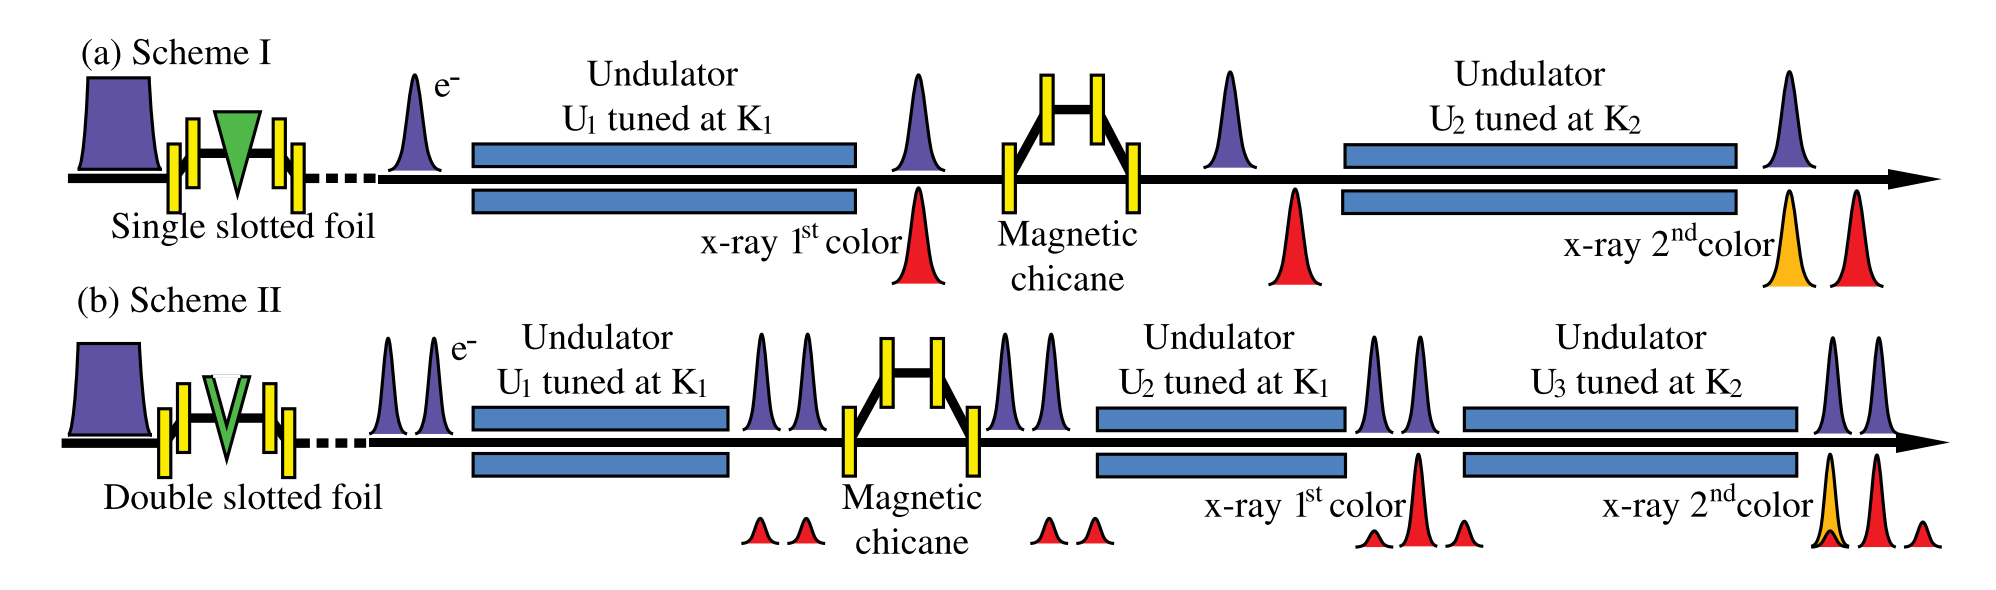
\includegraphics[width=1.00\textwidth]{images/Albertos-pump-probe-scheme.png}
	\caption[Schematic setup of an undulator based pump--probe scheme.]{Schematic setup of undulator parameter $K_{i}$ based pump--probe schemes at LCLS. Scheme I) creates one electron bunch using a single slotted foil and scheme II) creates two electron bunches using a double slotted foil. The electron bunches emit radiation with a wavelength depending on $K_{i}$. A time delay $\Delta t$ between pulses is introduced using a magnetic chicane. From \cite{Lutman-2013-PRL}. Reprinted with permission from APS.}
	\label{fig:Albertos-pump-probe-scheme}
\end{figure}
The first developed accelerator based X-ray pump--X-ray probe technique at LCLS \cite{Lutman-2013-PRL} uses a difference in undulator parameters, $K_{1,2}$, to create two pulses of different wavelength. The time delay is introduced through a magnetic chicane.\\[1\baselineskip]
%
A schematic setup is shown in Figure \ref{fig:Albertos-pump-probe-scheme}.
Following the figure to the top panel (a) Scheme I, one electron bunch is created through a single slotted foil\footnote{A single slotted foil or emittance-spoiling foil works similarly to a monochromator. It leaves a certain energy band of the electron bunch within the slot unspoiled and Coulomb scatters or spoils (compare to apertures) the rest. The 'dispersive' element is a magnetic chicane. By narrowing the electron beam one also reduces its pulse duration \cite{Emma-2004-PRL}.}. The use of the slotted foil enables control over the pulse duration. The electron bunch then travels through the undulator section $U_{1}$ tuned at strength parameter $K_{1}$ and is stimulated to lase, but the process does not go into saturation such that the electron bunch can be reused in the second undulator section. A magnetic chicane removes the microbunching from the section $U_{1}$ such that in undulator section $U_{2}$, tuned to undulator strength parameter $K_{2}$, the electron bunch lases again and the process is able to saturate. The maximal color separation between the two pulses is $~ 1.9\%$ in relative difference between $K_{1}$ and $K_{2}$.\\[1\baselineskip]
%
The time delay between the two pulses is introduced by a magnetic chicane that extends the pathway of the electrons and leaves photons unaffected. At LCLS, a dedicated chicane, for example, from the soft X-ray self-seeding instrument, can reach delays up to a maximum of $\SI{800}{\femto\second}$.
In this scheme, several factors prevent a minimal time delay, $\Delta t_{\text{min}}$, of zero. The minimal time delay opposed by the magnetic chicane, $\tau_{\text{min}}$, is dictated by the electron drift velocity mismatch to the speed of light. We can express that as,
\begin{equation}
\tau_{\text{min}} = \frac{l}{v_{\text{drift}}} - \frac{l}{c}\approx \SI{50}{\atto\second},
\label{eq:alberto-delta-t-min}
\end{equation}
with $l\approx \SI{4}{\meter}$ being the length between undulator sections $U_{1}$ and $U_{2}$, $c$ being the speed of light, and $v_{\text{drift}}$ being the drift velocity of the electron bunch. As the electron bunch drifts undeflected through the chicane close to the speed of light $\tau_{\text{min}}$ is typically on the tens of attoseconds timescale.
There is also a timing jitter between the two light pulses that is introduced by the magnetic chicane due to the magnetic field jitter and the electron beam energy jitter. The total contribution to the timing jitter is less than $0.4\%$ of the time delay imposed by the chicane. So, the delay chicane does not significantly contribute to the delay $\Delta t_{\text{min}}$. A bigger factor is the velocity mismatch of the light pulse and the electron bunch as they travel through a undulator section. This mismatch can be estimated by
\begin{equation}
\Delta t_{\text{min}}-\tau_{\text{min}}=\frac{N_{u} \lambda_{r}}{c},
\label{eq:alberto-beam-missmatch}
\end{equation}
with $N_{u}$ being the undulator periods. Given the parameters in study \cite{Lutman-2013-PRL}, $\Delta t_{\text{min}}=\SI{3}{\femto\second}$, such that a partial overlap between the electron bunch and light pulse could be achieved after the magnetic chicane. It should be noted that this scheme has been used in the described experiment.\\[1\baselineskip]
%
(b) Scheme II uses a double slotted foil\footnote{A double slotted foil works as a single slotted foil but it leaves two parts of the electron beam unspoiled through the two slots.} to create two electron beams. The two beams have a longitudinal separation that translates into the time delay. The electron bunches travel through a first set of undulators, $U_{1}$, that creates two pulses of the same wavelength. Due to the shortness of the section $U_{1}$, the lasing process does not saturate. The electron bunches are then delayed using a magnetic chicane such that the leading electron bunch overlaps with the trailing light pulse. This light pulse now functions as a seed for the leading electron bunch such that this pulse saturates in undulator section $U_{2}$. The electron bunches then travel through the magnets at $U_{3}$, where the trailing electron bunch creates a second saturated pulse. The leading electron bunch barely emits radiation in $U_{3}$ since its energy spread has become too large after lasing in $U_{2}$. Using this scheme, two saturated, lasing pulses can be generated; however, temporal overlap cannot be achieved.
%
%
%
%
\subsubsection{The Twin bunch or Lorentz factor based pump--probe scheme}
\begin{figure}
	\centering
		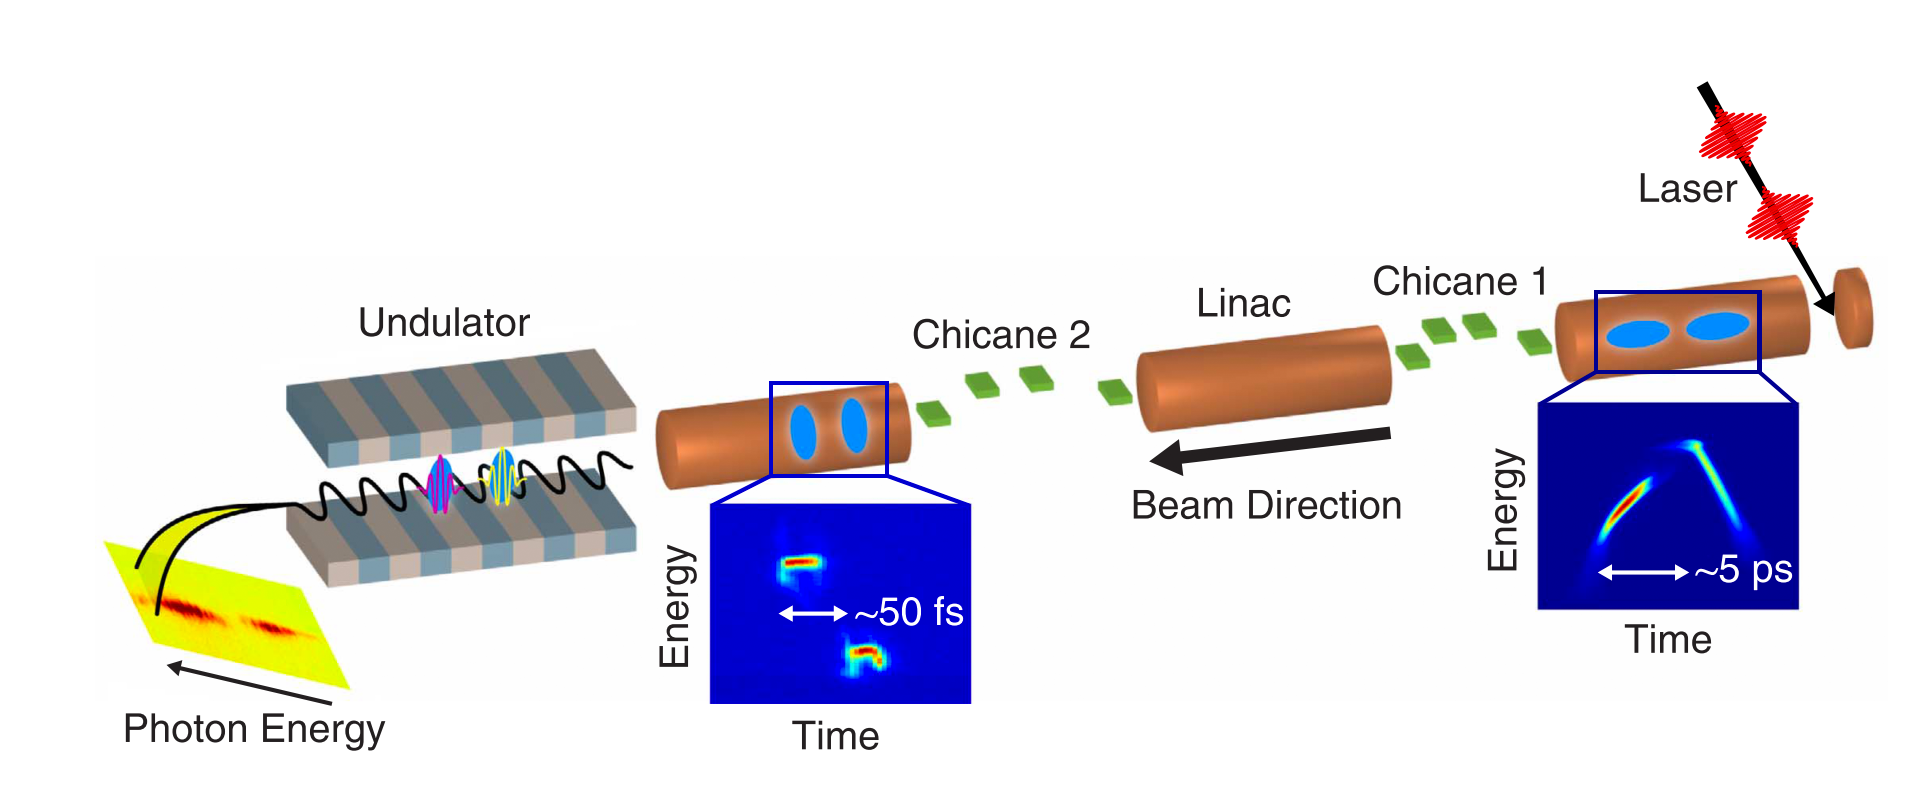
\includegraphics[width=1.00\textwidth]{images/Agos-pump-probe-scheme.png}
	\caption[Schematic setup of a bunch based pump-probe setup.]{Schematic setup of the two bunch, two color pump--probe setup at LCLS. Two laser pulses shot at a cathode create two electron bunches with a delay $\Delta t$ on the picosecond timescale. Two magnetic chicanes compress the bunches such that a delay $\Delta t$ is on the ten femtosecond timescale. Both pulses go through one undulator section and the lasing process is saturated. The relative color separation is on the order of $1\%$ between the bunches. From \citep[\href{http://creativecommons.org/licenses/by/4.0/}{\ccby}]{Marinelli-2015-NatComm}.}
	\label{fig:Agos-pump-probe-scheme}
\end{figure}
The second developed accelerator-based X-ray pump-X-ray probe technique at LCLS \cite{Marinelli-2015-NatComm} uses two electron bunches of different energy. A schematic setup of this beam operation can be found in Figure \ref{fig:Agos-pump-probe-scheme}. The electron bunches are created through a double laser pulse that impinges on a photocathode. Initially, these two bunches are delayed by a few picoseconds, however, two magnetic chicanes compress the electron bunches in the time and intensity domain such that a time delay on the ten-femtosecond timescale is achieved. The electron bunches then travel through one undulator section and both pulses saturate in their lasing process. At $8.3k$ eV, both pulses combined can reach pulse energies of $1.2mJ$, the color separation is $100$ eV and the time separation ranges from $\Delta t_{min}=0fs$ to $\Delta t_{max}=100fs$. For hard X-rays, this method requires the pump-pulse to have a higher photon energy than the probe-pulse, although their respective intensities may vary. However, this method is not restricted to hard X-rays and can be utilized with soft X-rays. In soft X-rays, the slotted spoiler foil can be used. This enables further control over the electron bunches and allows crossing time zero with both pulses.
%%%
\section{Rare-gas clusters}\label{sec:cluster-theory}
%%%%%%%%
%- Why are rare gas clusters a suitable sample
%%%%%%%%
Clusters have a long history as samples to study the light-matter interaction for a few reasons. Their characteristics are well known, they can form interesting states, and they often have practical purposes \cite{Haberland-1994-Springer}. Generally speaking, clusters are an aggregation of atoms or molecules and vary in size. Their size ranges from a few atoms to mesoscopic sizes such that one can classify a cluster as a bulk material. Even though clusters can form exotic materials that are interesting to study, they can be simulated with computer models. Besides these testbed characteristics, clusters can be created relatively easily and are tunable in size. Rare-gas clusters are a subclass of clusters and they are bound by van der Waals forces, thus are normally neutral-charged. Single van der Waals clusters typically form in an icosahedral\footnote{An icosahedron is a polyhedron with 20 faces, i.e., a dice with 20 faces.} shape when they are sufficiently small (up to nanometer sized) \cite{Miehle-1989-JCP} and have mostly a fcc-crystal\footnote{fcc is an acronym for face-centered cubic. A very common crystal structure.} structure but exhibit also hcp-crystal\footnote{hcp stands for hexagonal close-packed and is also a crystal structure.} structures \cite{VanDeWaal-1993-JCP,Krainyukova-2006-TSF}. In the present work, superfluid helium clusters (or droplets), solid xenon clusters and a mixture of both have been used as a sample. Therefore, we shall explore the creation of homogenous and heterogeneous rare-gas clusters in the next sub-sections.
%
%
%
\subsection{Generation of homogenous clusters}\label{sec:homogenous-cluster}
%%%%%%
%- the theory behind rare-gas cluster creation.
%%%%%%
Rare-gas clusters, for example xenon clusters, can be generated in a variety of ways. Often, as in the described experiment, rare-gas clusters are created by releasing gas from a reservoir into a vacuum. Here, a nozzle connects the gas reservoir with the vacuum system and while the gas is expanding through the nozzle, many collisions take place. So, the cluster formation process can be explained intuitively through a kinetic model \cite{Lippmann-1984-JCP}. In other words, clusters grow through collisions with monomer, dimer and other clusters. We can express a collision squence mathematically through the following reaction formula
\begin{align}
A_{n}+A_{m} \rightleftharpoons A_{n+m}^{*},\quad n,m=1,2,...,\quad \text{collision,}
\intertext{with $n,m$ denoting the number of monomer assembling body $A_{n,m}$. A body $A_{n}$ collides with another body $A_{m}$ and forms a metastable state $A_{n+m}^{*}$ that will dissociate if no subsequent collision deactivates it}
A_{n+m}^{*}+M\rightleftharpoons A_{n+m} + M,\quad \mathrm{activation/deactivation.}
\label{eq:early-cluster-growth}
\end{align}
$M$ is a chaperone that can be any kind of third body that removes energy from the system. Note that a chaperone $M$ can also activate the state again.\\[1\baselineskip]
%
While the early stage of the cluster growth is driven by the monomer addition, cluster-cluster coagulation starts to dominate the later growth processes \cite{Zurek-1980-JCP,Soler-1982-PRL}. This is due to the quantitative increase in small clusters in the generation process that then start to collide, similar to the above kinetic model. From empirical evidence, we know that clusters solely generated through monomer addition have a size distribution of an exponential decay with a rather large decay constant, whereas larger clusters that grew through coagulation follow a log-normal distribution. In other words, the density of smaller clusters including monomers and dimers decreases as larger clusters are formed of these particles through coagulation. The most probable size of a cluster, i.e., the maximum of the log-normal distribution, is given by the parameters of the supersonic gas expansion, which is what we will discuss next.\\[1\baselineskip]
%
\begin{figure}
	\centering
		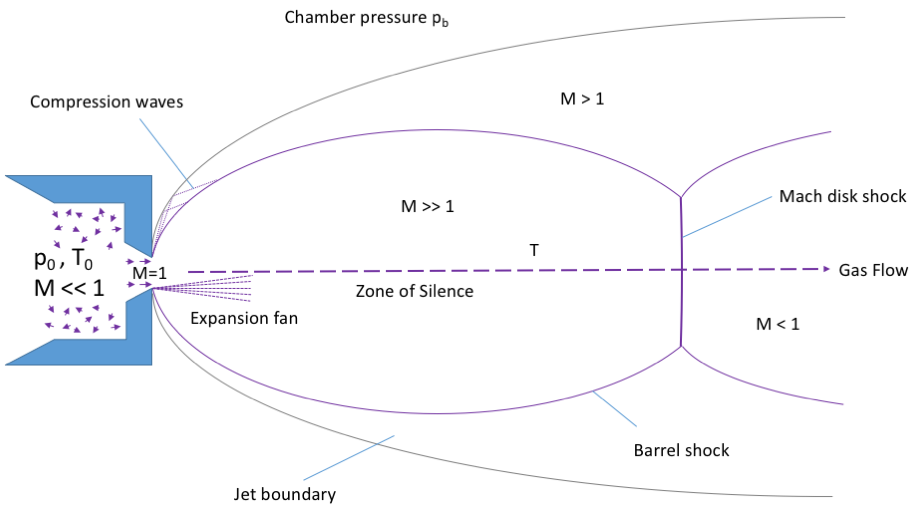
\includegraphics[width=0.85\textwidth]{images/freeJetExpansion.png}
	\caption[Schematic of a supersonic gas expansion into a vacuum.]{Schematic of a supersonic gas expansion into the vacuum. Gas is stored in a reservoir at pressure $p_{0}$, temperature $t_{0}$ and speed of the gas is thermally distributed $\left(M\ll 1\right)$. As the gas enters the nozzle area, it is accelerated to the speed of sound $\left(M=1\right)$ and as the gas expands, the temperature T drops altering the speed of sound such that the gas now travels supersonically $\left(M\gg 1\right)$. In this expansion, clusters are generated in the nozzle region, where $M=1$ (see text for details). After \citep{Miller-1988-Oxford}.}
	\label{fig:freeJetExpansion}
\end{figure}
%
Supersonic jet setups typically store gas in a reservoir at a certain stagnation pressure, $p_{0}$, and temperature, $T_{0}$. The gas expands through a nozzle into a vacuum and Figure \ref{fig:freeJetExpansion} shows a schematic drawing of this process. Typical values for $p_{0}$ are 10 bars, where the mean free path of the atoms is much smaller than the nozzle diameter, d\footnote{A schematic drawing of the nozzle can be found in Figure \ref{fig:parker-valve}. See also Equation \eqref{eq:equivalent-nozzle-opening} for non-pinhole nozzle openings.}. This is why many collisions occur during the expansion in the nozzle and the above described kinetic theory explains the cluster formation. However, this does not hold true in the supersonic molecular flow region, where no further cluster growth happens. To understand the expansion process in detail, we assume an ideal gas. To describe the gas expansion itself, we further assume that no clusters are formed and that turbulence and the effects of heat conduction are unimportant \cite{Yamada-2001-SciDir,Haberland-1994-Springer}.\\[1\baselineskip]
%
To begin, the velocity distribution of the gas is thermally distributed at a set temperature $T_{0}$. The movement direction of each atom is randomly orientated. For an ideal gas, we can define the enthalpy, $H_{0}$, in the stagnation chamber by
\begin{align}
H_{0}=C_{P}\ T_{0},
\intertext{with the specific heat at constant pressure, $C_{P}$, for atoms}
C_{P}=\frac{5}{2}k_{B},
\label{eq:stagnation-enthalpy}
\end{align}
where $k_{B}$ is the Boltzman constant. The expansion of the gas through the nozzle is driven by the pressure difference $p_{b}/p_{0}$. In the nozzle, the steady gas flow becomes directed and the enthalpy, $H_{0}$, is converted into kinetic energy $\frac{1}{2}m v^{2}$ and a remaining enthalpy, $H$. So, in the expansion process, we can use the conservation of energy and Equation \eqref{eq:stagnation-enthalpy} to write down
\begin{equation}
H_{0}=H+\frac{1}{2}m_{gas} v^{2} = C_{P}\ T+\frac{1}{2}m_{gas}v^{2},
\label{eq:local-temperature}
\end{equation}
with $T$ being the local temperature along the gas flow and $m_{gas}$ the atomic mass of the gas. To simplify, let us define the Mach number, $M$, as the ratio of the stream velocity, $v$, and the local speed of sound, $c_{s}$. We can express the local speed of sound as
\begin{equation}
c_{s}=\sqrt{\frac{\gamma k_{B} T}{m_{gas}}},
\label{eq:local-speed-of-sound}
\end{equation}
with the ratio of specific heats $\gamma = \frac{C_{P}}{C_{V}}$ at constant pressure and volume. $\gamma$ can be regarded as independent of temperature for atomic gases and we can rearrange Equation \eqref{eq:local-temperature} to 
\begin{equation}
T=T_{0}\left(1+\frac{1}{2}\left(\gamma - 1\right)M^{2}\right)^{-1}.
\label{eq:local-temperature-definition}
\end{equation}
Here the interplay between the Mach number and the local temperature give insight into the directed mass flow versus the remaining thermal energy in the system. As indicated in the Figure \ref{fig:freeJetExpansion}, M increases dramatically along the expansion axis and that is due to decrease in $c_{s}$, which is proportional to $\sqrt{T}$ as indicated in Equation \eqref{eq:local-speed-of-sound}. The gas quickly reaches the terminal velocity while the speed of sound is decreasing. We may write the terminal velocity as
\begin{equation}
v_{\infty}=\sqrt{\frac{2 R}{m_{gas}}\left(\frac{\gamma}{\gamma-1}\right) T_{0}},
\label{eq:terminal-velocity}
\end{equation}
with $R$ being the universal gas constant. The expansion speed of the gas gives the name to such types of gas sources, namely supersonic jets. This equation is also useful to calculate gas or cluster flight times -- $t_{\text{flight}}=\frac{D}{v_{\infty}}$ -- if the distance $D$ from nozzle to interaction point is known (see Section \ref{sec:jet-timing}). \\[1\baselineskip]
%
Let us describe the appearance of the jet stream (see Figure \ref{fig:freeJetExpansion}) next \citep{Miller-1988-Oxford}. Upon exiting the nozzle, the Mach number increases by a wide margin ($M\gg 1$). This means that the gas travels faster than information in this medium. Here, a \textit{zone of silence} is formed, where the gas flow is not influenced by other particles or boundary conditions. As the supersonic flow exits the nozzle, it has to turn around the edge of the nozzle to further expand and it does so by actually creating smaller Mach waves. At the borders of the zone of silence, $M$ decreases drastically, resulting in dense regions that are called \textit{barrel shock} to the sides and \textit{Mach disk shock} downstream the gas flow. For an unhindered transport of the gas and clusters to the interaction region, the interaction region needs to be within the zone of silence. We can express the distance from the nozzle to the Mach disk $x_{MD}$ through
\begin{equation}
\frac{x_{MD}}{d}=0.67\sqrt{\frac{p_{0}}{p_{b}}},
\label{eq:distance-of-mach-disk}
\end{equation}
with the nozzle diameter $d$. So the competing stagnation pressure $p_{0}$ and the background pressure $p_{b}$ define the distance of the otherwise static parameters. $p_{b}$ needs to be low enough to drive the Mach disk downstream of the interaction region. By using skimmers and thereby physically separating the jet expansion into separately pumped compartments, the background pressure $p_{b}$ can be reduced, hence $x_{MD}$ increased.\\[1\baselineskip]
%
While we have described a cooling gas in the expansion process it should be noted that the clusters are comparably hot. Through the kinetic process described above, they are efficiently heated. The two processes to lose energy are, one, collisions with a chaperone $M$ that deactivates the cluster, or two, evaporation of monomers from the cluster. The evaporation process makes the temperature size-independent, after the clusters have reached a certain minimum size \cite{Farges-1981-SurfSci}. Typically, the jet reaches temperatures of a few Kelvin and the cluster temperature is heavily dependent on their material, particularly the dissociation energy. Relevant for this study are the temperature of Xenon cluster, which is $\sim 75K$\footnote{To put this temperature in perspective, krypton clusters are $~50K$ and argon clusters $~40K$ \citep{Farges-1981-SurfSci,Gspann-1986-Springer}. Note that in this study the cluster size was $\bar{N} > 800$, hence above the minimum value to be size independent. For the evaporative cooling process to settle at a given temperature, a certain flight distance (in the cited study 6.5 cm) should also be taken into account.}, and the fact that xenon clusters are solid as their melting temperature is higher \cite{Gspann-1986-Springer}. For similar reasons, helium clusters are liquid, which is why they are often called (helium-)droplets. If helium droplets are produced using a cryogenic jet even superfluid helium-droplets can be observed.\\[1\baselineskip]
\begin{table}
	\centering
		\begin{tabular}{ | l | l | l | l | l | }
			\hline
			Helium & Neon & Argon & Krypton & Xenon \\ \hline
			3.85 & 185 & 1646 & 2980 & 5554 \\ \hline
		\end{tabular}
	\caption[Parameter $K_{\text{gas}}$ values for rare-gases.]{Parameter $K_{\text{gas}}$ values for rare-gases \cite{Schorb-2012-Thesis}.}
	\label{tab:k-parameter}
\end{table}
At the current point of the discussion, it should be apparent that the average cluster size\index{cluster size} is very much dependent on the gas type, stagnation temperature $T_{0}$, stagnation pressure $p_{0}$ and the nozzle diameter. Indeed, an empirically found scaling law\index{scaling law}, named after Hagena\index{Hagena|see {scaling law}} \cite{Hagena-1972-JCP,Hagena-1981-SurfSci,Hagena-1987-ZeitschriftAMC}, can be written down as
\begin{equation}
\Gamma^{*} = K_{\text{gas}} \cdot T_{0}^{0.25x-1.5} \cdot p_{0} \cdot d_{eq}^{x}\quad \left[\frac{\text{$\mu$m mbar}}{\text{K}}\right],
\label{eq:Hagena-parameter}
\end{equation}
with the gas-specific parameter $K_{\text{gas}}$ that can be found in Table \ref{tab:k-parameter} for some rare-gases, the gas specific parameter $x$ that varies between 0.5 and 1 and is 0.85 for all rare-gases, and the equivalent nozzle opening, $d_{eq}$, that is $d_{eq}=d$ for pinhole sources and for conical nozzles $d_{eq}$ becomes \citep{Schorb-2012-Thesis}
\begin{equation}
d_{eq} = d\frac{\tan\left(\Phi_{0}\right)}{\tan\left(\Phi\right)} = 0.719 \frac{d}{\tan\left(\Phi\right)}
\label{eq:equivalent-nozzle-opening}
\end{equation}
with the half opening angle of the nozzle $\Phi$ and the half opening of the free gas expansion $\Phi_{0}$. The Hagena scaling parameter $\Gamma^{*}$\index{Hagena!scaling parameter} allows us to estimate the mean cluster size, i.e., amount of accumulated particles per cluster $<N>$, as follows
\begin{itemize}
	\item $\Gamma^{*} < 350$, no cluster formation is observed;
	\item $350 < \Gamma^{*} < 1800$, in this region $<N>$ reads
		\begin{equation}
		<N> = 38.4 \left(\frac{\Gamma^{*}}{1000}\right)^{1.64};
		\label{eq:intermediate-hagena-scaling}
		\end{equation}
	\item $1800 < \Gamma^{*}$, in this region $<N>$ is
		\begin{equation}
		<N> = 33.0 \left(\frac{\Gamma^{*}}{1000}\right)^{2.35}.
		\label{eq:large-hagena-scaling}
		\end{equation}
\end{itemize}
Supersonic jets generally create clusters of different sizes. This size distribution is centered around $<N>$ and for solid rare-gas clusters this distribution is a log-normal distribution. The size distribution can be an experimental challenge, especially when size dependent effects are investigated. Historically, electron diffraction \cite{Farges-1981-SurfSci,Bartell-1986-ChemRev} has been used to determine the mean cluster size, mean temperature and mean geometry. Today, free electron lasers allow the determination of the size of a single cluster through a diffraction image, and by measuring enough single clusters, one can reproduce size distributions of a supersonic jet as shown in Figure \ref{fig:size-distributions}.\\[1\baselineskip]
Experiments using supersonic jets for cluster generation are typically performed with pulsed valves to decrease cost and gas load in the overall system. Upon opening and closing of the valve, the gas density varies. This mostly affects the cluster size and one would expect to see smaller clusters. This remains true in the beginning of the pulse but in the \textit{afterpulse}\index{afterpulse} one finds giant clusters that exceed the above-described scaling laws due to the effects when closing the valve \cite{Rupp-2014-JCP}.
%
%
%
%
%
\subsection{Creation of heterogeneous clusters: The pickup principle}\label{sec:heterogeneous-cluster}
%%%%%%%%%%%%%%%%%
%- Heterogeneous clusters, e.g. He Xe\\
%- Do you have literature on that?
%%%%%%%%%%%%%%%%%
\begin{figure}
	\centering
		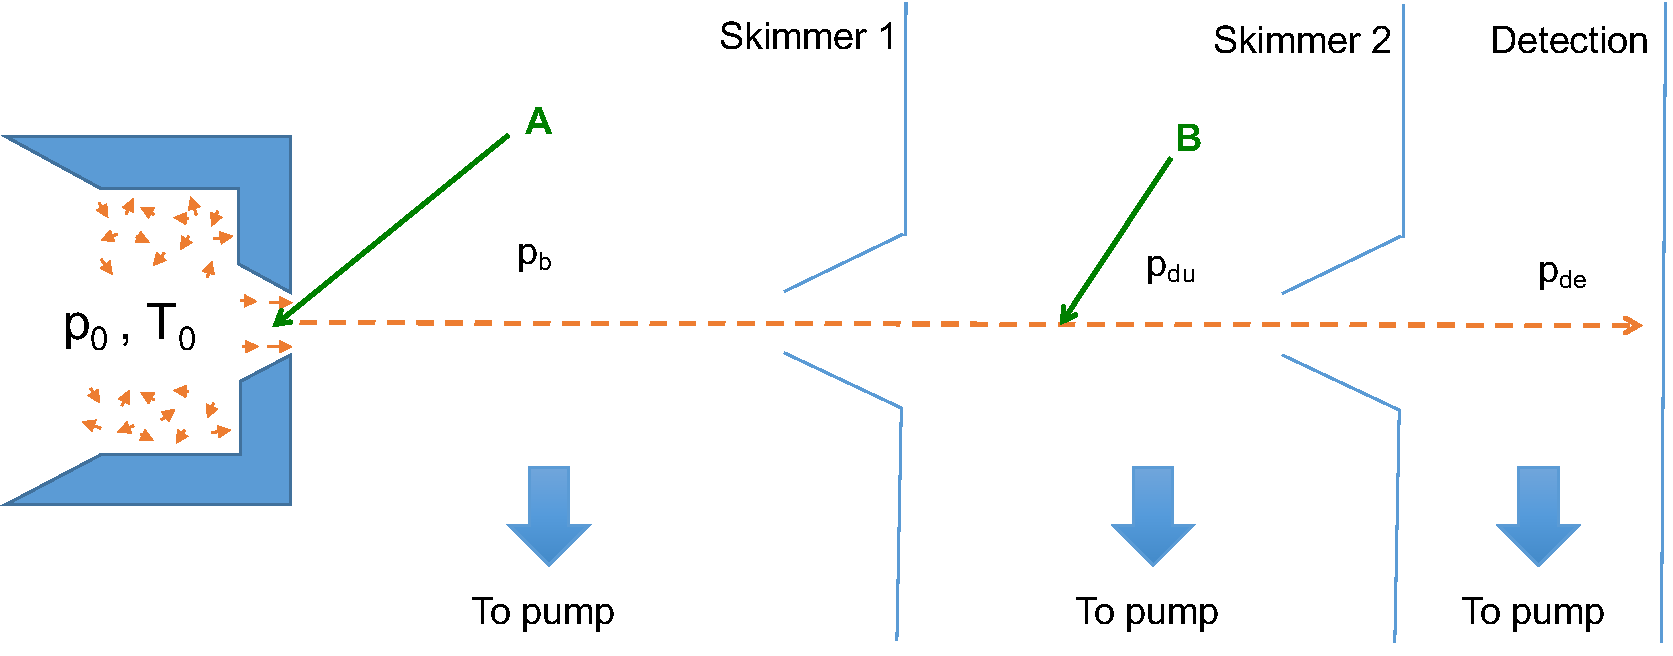
\includegraphics[width=0.80\textwidth]{images/pick-up.pdf}
	\caption[Schematic of a pickup (gas-)source.]{Schematic setup to generate heterogeneous clusters through pickup. Thereby is a cluster generated via supersonic gas expansion, which is doped at regions marked A or B. In region A, the dopant gas is mixed in the nozzle such that it becomes part of the nucleus. In region B, the cluster condenses atoms on its surface from the background gas of pressure $p_{\text{du}}$. The cluster can be detected upon evaporation, e.g., due to contact with the chamber, through the pressure $p_{\text{de}}$. After \cite{Gough-1985-JChemPhys,Haberland-1994-Springer}.}
	\label{fig:pickupPrinciple}
\end{figure}
A possibility to create heterogeneous clusters is through the principle of picking-up atoms or molecules \cite{Gough-1985-JChemPhys,Haberland-1994-Springer}. Figure \ref{fig:pickupPrinciple} illustrates pickup regions that are typically used in an experiment. Mainly, there are two different pickup places, one, monomers are added to the cluster in region A of Figure \ref{fig:pickupPrinciple} that represents the nozzle of a supersonic source, or two, they can be picked up by a cluster in region B for example through an increased background pressure $p_{b2}$ with the dopant material. If clusters pick up atoms or molecules in the nozzle region A, they can become part of the cluster formation and can be found inside of solid clusters. If atoms or molecules are picked up in region B, they stick to the surface of solid clusters. If a (super-)liquid cluster picks up a dopant, it may move within the droplet. Since the traversing cluster is much larger and heavier than a colliding monomer, the trajectory is not affected significantly. Already pressures of $p_{b2}=10^{-11}$ bar over a pickup length of a few centimeters can dope the cluster significantly. At these low pressures, picking up atoms or molecules in region B requires less gas load on the system but is also less efficient than picking up in region B. To increase the pickup levels in region B, a gas cell can be used as much higher pressures can be achieved within the gas cell without putting too much gas-load on the overall system. In this work, gaseous xenon was picked up by superfluid helium droplets in region B. To understand doping levels, the following considerations are helpful.\\[1\baselineskip]
%
The collision with the cluster and a dopant\index{dopant} does add energy to the cluster, as does the cluster growth process itself. This is why the initial cluster will lose particles through evaporation upon pick up of a dopant \citep{Gomez-2011-JCP}. The loss of particles through evaporative cooling is dependent on the ratio of dissociation energies of the two materials and can be expressed as
\begin{equation}
N_{\text{Evaporated from cluster}} \approx \frac{\epsilon_{\text{cluster}}}{\epsilon_{\text{dopant}}},
\label{eq:evaporated-amount}
\end{equation}
with the dissociation energy of the cluster $\epsilon_{\text{cluster}}$ and of the dopant $\epsilon_{\text{dopant}}$. In the case where a helium droplet is doped with xenon atoms, we may use the dissociation energies of helium, $\epsilon_{He}\approx 0.6\cdot 10^{-3}$ eV, and xenon, $\epsilon_{Xe}\approx 0.15$ eV \citep{Gomez-2011-JCP,Gomez-2014-Science}, to conclude that approximately 250 helium atoms evaporate by picking up 1 xenon atom.\\[1\baselineskip]
%
Now we can extend this idea to estimate the number of picked-up atoms, if we were to know the number of atoms in the cluster before and after the pickup area. An estimate of the initial cluster size $\left\langle N_{\text{cluster}}\right\rangle$ can be reached through the scaling laws\footnote{As already established the actual cluster size produced with a supersonic jet will vary, hence the average cluster size $\left\langle N_{\text{cluster}}\right\rangle$.} as discussed in Section \ref{sec:homogenous-cluster}. An estimate of the cluster size after the pickup can be established through measuring the partial pressure of the cluster material without the pickup, $p_{\text{de}}$, for example, in the detection chamber when the particle jet hits a wall and evaporates\footnote{For example with a residual gas analyzer.} (see Figure \ref{fig:pickupPrinciple}), and the partial pressure with pickup, $\Delta p_{\text{de}}$. The relative difference $\tfrac{\Delta p_{\text{de}}}{p_{\text{de}}}$ then scales with
\begin{equation}
\left\langle N_{\text{dopant}}\right\rangle \approx \frac{\epsilon_{\text{cluster}}}{\epsilon_{\text{dopant}}} \cdot \frac{\Delta p_{\text{de}} \left\langle N_{\text{cluster}}\right\rangle}{p_{\text{de}}},
\label{eq:average-dopant}
\end{equation}
and the amount of picked up atoms, $\left\langle N_{\text{dopant}}\right\rangle$, can be estimated on average.
%%%
%\section{Introduction into X-ray scattering}\label{sec:scattering-theory}
%%%%%%%%%%%%%%%%%%%%%
%- Starting with Maxwell equations (this would be coming from the far end, I might be able to go into Guiniers formalism earlier. Depending on space.)\\
%- Mathematical model for electromagnetic wave\\
%- Kramers-Kronig relations\\
%- Mie scattering in a nutshell
%%%%%%%%%%%%%%%%%%%%%%%
%
\section{Soft X-rays in matter}\label{sec:light-matter-interaction}
%We may break down the light-matter interaction into five categories, 1) coherent-elastic scattering (see sub-Section \ref{sec:saxs}), 2) resonant processes (absorption, see sub-Section \ref{sec:absorption}), 3) incoherent scattering (Compton effect), high-energy physics effects of 4) pair production, and 5) absorption effects with the nucleus. The effects are dependent on the wavelength and the cross-sections for  effects 3-5 are so small that they can be neglected in the soft X-ray regime. We will therefore concentrate the following sub-sections on points 1-2 and restrict ourselves to the for the experiment necessary theory.
When light interacts with a nanoparticle it either scatters or is absorbed. Although XFEL are intense lightsources, we can reduce the considerations in this section to the elastic and coherent scattering as well as relevant resonant effects. The Section \ref{sec:saxs} discusses the scattering of an electron and extends this concept to the scattering and imaging of a nanoparticle. The Section \ref{sec:absorption} discusses several effects due to absorption and the Section \ref{sec:relaxation} discusses effects that occur after the absorption of a photon. This way, we follow the discussion in \citep{Als-Nielson-2011-JWS} and avoid effects that have negligible cross-sections such as the Compton effect, the pair-production, and the scattering from the nucleus. 
%This section will give  a brief introduction into the elastic scattering of X-rays with matter. The actual scattering process is very complex as it is an interplay of coherent, incoherent and elastic, inelastic processes. Fortunately, we can reduce the scattering description to its main process: The coherent and elastic scattering. In other words, we neglect Compton scattering (incoherent), any kind of absorption processes (inelastic) and effects form the scattering of multiple particles. We will then start this section by looking at the small angle scattering of atoms and continue on to extended objects such as clusters. The section is rounded off by an introduction to the inverse problem and basic algorithm ideas to overcome the issue of phase retrieval.
%Photons can also be absorbed by atoms in which case an electron get either excited to another state or ionized. At X-ray wavelengths matter typically gets ionized in the inner shells. Upon absorption a cascade of relaxation processes begins and the now ionized atom finds the new most energetic favorable state. These processes are particularly dependent on the wavelength of the incident photons but also the type of atom. This chapter is devoted to these processes and particular the absorption process is described in Section \ref{sec:absorption} and the relaxation processes in \ref{sec:relaxation}.
%
%
%
\subsection{Diffractive imaging}\label{sec:saxs}
%%%%%%%%%%
%- Switch to Guiniers approximation and description\\
%- Work towards small angle scattering of small particles\\
%- Particular spheres\\
%- Discuss extreme positions
%%%%%%%%%%%
When light interacts with nanoobjects the fundamental scatterers are electrons. Let us first consider the scattering of an electron as a result of being accelerated in an electro-magnetic field, i.e., a light wave. Then, we proceed to the scattering of an atom followed by the scattering of an extended object with a continuous electron density.\\[1\baselineskip]
%We can describe an electric field of a light wave semi-classically via the following expression \citep{Als-Nielson-2011-JWS}
%\begin{equation}
%\vec{E}(\vec{r},t) = \vec{\epsilon} E_{0} e^{i \left(\vec{k}\cdot\vec{r}-\omega_{0}t\right)},
%\end{equation}
%with $\vec{r}$ the Cartesian coordinate vector, $\hbar \vec{k}$ the momentum of a photon, $\hbar \omega_{0}$ the energy of a photon, $E_{0}$ the incident amplitude, and \vec{\epsilon} an unit vector due to the polarization. $\vec{\epsilon}$ obeys $\vec{\epsilon}\cdot\vec{k}=\vec{k}\cdot\vec{E}=\vec{k}\cdot\vec{B}=0$, with the magnetic field $\vec{B}$, as the electro-magnetic waves are transverse. To avoid delving into a quantum mechanic description, we shall call \vec{k} the wavevector.
Let us intriduce the electric field of an incident wave $E_{in}=E_{0}e^{-i\omega t}$ that will irradiate an electron. The electron is accelerated in this electric field and will thus start to emit radiation similarly to a small dipole antenna. We can write this radiated electric field as \citep{Als-Nielson-2011-JWS}
\begin{equation}
E_{rad}(R,t)=-\underbrace{\left(\frac{e^2}{4\pi \epsilon_0 m c^2}\right)}_{r_{0}}\ E_{in}\ \frac{e^{i k R}}{R} \cos\left(\psi\right),
\label{eq:radiated-by-electron}
\end{equation}
with $k$ being the usual wave-number, $R$ being the distance from the source of radiation, $\psi$ being the observation angle, and $r_0$ being the \textit{Thomson scattering length}, or the \textit{classical electron radius}. $r_0$ can be written in practical units as
\begin{equation}
r_0 = \frac{e^2}{4\pi \epsilon_0 m c^2} = 2.82\cdot 10^{-5}\si{\angstrom},
\label{eq:thomson-scattering-length}
\end{equation}
where $-e$ is the charge of the radiating electron, $m$ is the mass of the electron, $c$ is the speed of light, and $\epsilon_0$ is the permittivity of free space.\\[1\baselineskip]
%
Now we would like to understand the cross-section of this scattering process better. We can establish a \textit{differential cross-section}, $\left(\tfrac{d\sigma}{d\Omega}\right)$, which follows the same concept of the already discussed example in Equation \eqref{eq:absorption-cross-section}. The only difference is that we now consider a scattered intensity, $I_{sc}$, of an incident flux, $\left(I_{0}/A_{0}\right)$, into a solid angle, $\Delta \Omega$. We may express this as
\begin{align}
\left(\frac{d\sigma}{d\Omega}\right)&=\frac{I_{sc}}{\left(I_{0}/A_{0}\right)\Delta\Omega}=\frac{\left|E_{rad}\right|^2 R^2}{\left|E_{in}\right|^2}=r_0^2 \cos^{2}\left(\psi\right).
\label{eq:scattering-crosssection}
\end{align}
By integrating over the full angular space, the total cross-section of the scattering of an electron, $\sigma_{T}$, results in
\begin{align}
\sigma_{T} = \left(\frac{8\pi}{3}\right) r_{0}^{2} = \SI{0.665}{\barn}
\label{eq:Thomson-cross-section}
\end{align}
%\begin{align}
%\left(\frac{d\sigma}{d\Omega}\right)&=\frac{\left(\text{Number of X-rays scattered per second into $\Delta \Omega$}\right)}{\left(\text{Incident flux}\right)\left(\Delta\Omega\right)}=\frac{I_{sc}}{\left(I_{0}/A_{0}\right)\Delta\Omega},
%\label{eq:scattering-crosssection}
%\end{align}
%with $A_{0}$ being the covered area of the incident beam. If an electro-magnetic wave encounters an electron, we can describe the scattering semi-classical by imagining how an electron starts to oscillate once it sees an incoming electric wave. The electron then functions as a dipole antenna eventually radiating the wave into a certain solid angle $\Delta \Omega$. Depending on the polarization of the incident beam we can reduce Equation \eqref{eq:scattering-crosssection} to \citep{Als-Nielson-2011-JWS}
%\begin{align}
%\left(\frac{d\sigma}{d\Omega}\right)&=r_{0}^{2}P,
%\intertext{with the classical electron radius $r_{0}=2.82\ 10^{-5}\text{\AA}$ and the polarization factor P}
%P&=\begin{cases}
%1& \text{vertical scattering plane},\\
%\cos^{2}\left(\Psi\right)&\text{horizontal scattering plane}, and\\
%\frac{1}{2}\left(1+\cos^{2}\left(\Psi\right)\right)& \text{unpolarized source.}
%\end{cases}
%\end{align}
We can now move on and use this knowledge for atoms, where we have Z electrons. To describe electrons in an atom, let us introduce an electron density $\rho_{e}\left(\vec{r}\right)$ that describes the probability density of electrons in an atom. Figure \ref{fig:X-ray-scattering} illustrates the scattering process by one atom. An incident beam, with wave vector $\vec{k}$, is elastically scattered at a point $\vec{r}$ into a wave with $\vec{k}'$ such that $\left|\vec{k}\right|=\left|\vec{k}'\right|$. As the illustrated waves are scattered at different points, they have an optical path difference of $2 \delta$. This difference in path length results in a phase difference in the wavefront, which leads to interference. We can describe this phase difference, $\Delta \Phi\left(\vec{r}\right)$, of the waves scattered at $\vec{r}$ and the origin by
\begin{equation}
\Delta \Phi\left(\vec{r}\right) = \left(\vec{k}-\vec{k}'\right)\cdot \vec{r} = \vec{Q} \cdot r,
\label{eq:phase-difference}
\end{equation}
with $\vec{Q}$ being denoted as the \textit{wave-vector transfer}\index{wave vector!transfer}. Through trigonometry, we can establish the more common denotation of the wave-vector $\vec{Q}$
\begin{equation}
\vec{Q}=2 \left|\vec{k}\right| \sin\left(\frac{\Theta}{2}\right)=\frac{4 \pi}{\lambda}\sin\left(\frac{\Theta}{2}\right),
\label{eq:Q-scattering-angle}
\end{equation}
with the wavelength of the light $\lambda$ and the scattering angle $\Theta$.\\[1\baselineskip]
\begin{figure}
	\centering
		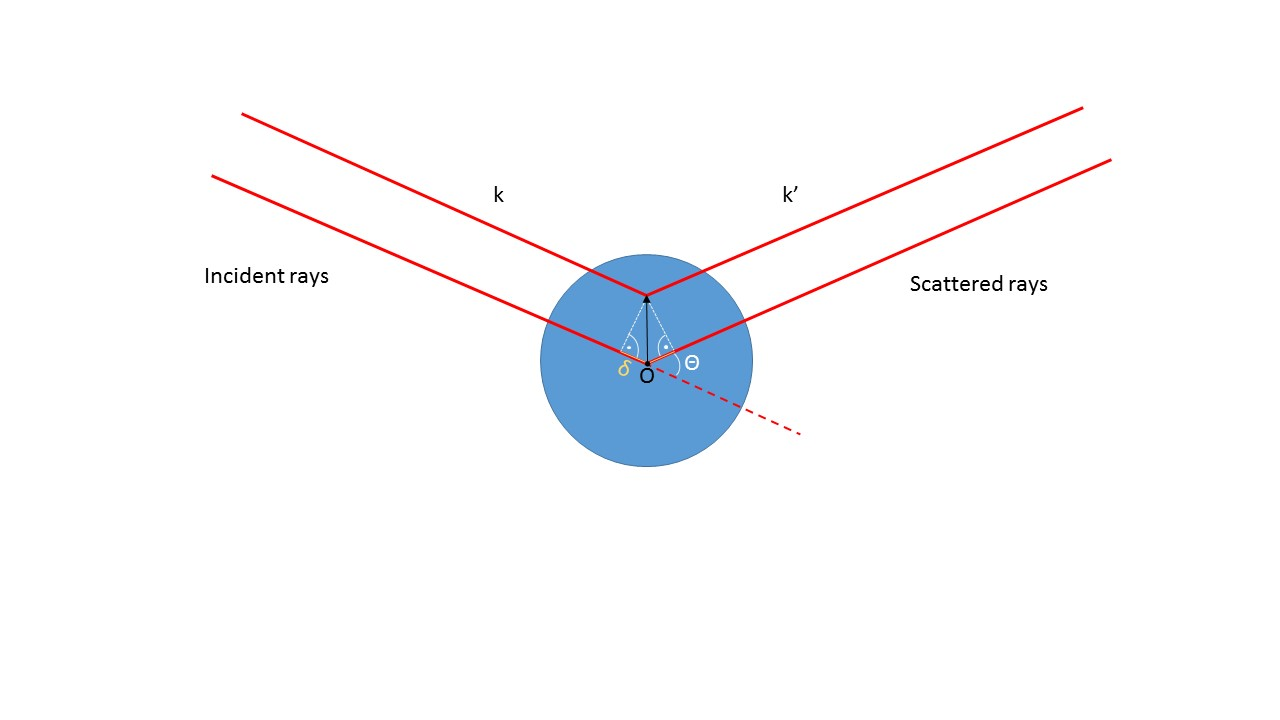
\includegraphics[width=1.00\textwidth]{images/X-ray-scattering.jpg}
	\caption[Principle of scattering rays of an atom.]{Principle of scattering rays of an atom. After \cite{Als-Nielson-2011-JWS,Guinier-1955-JWS}.}
	\label{fig:X-ray-scattering}
\end{figure}
%
A volume element $d\vec{r}$ of the atom at $\vec{r}$ will now scatter proportional to its electron density, namely by $-r_{0}\rho\left(\vec{r}\right)d\vec{r}$. At scattering angle $\Theta=0$, i.e., $\vec{Q}=0$ the \textit{atomic scattering factor}, $f^{0}$, is
\begin{equation}
f^{0}\left(\vec{Q}\rightarrow 0\right)=Z,
\label{eq:transform-number-of-particles}
\end{equation}
because all scatterers are in phase. As we increase the angle $\Theta$, the phase difference, $\Delta \Phi\left(\vec{r}\right)$, leads to interference. We can describe this by multiplying a phase factor $e^{i \vec{Q}\cdot \vec{r}}$ to the contribution of the scattered field, $-r_{0}\rho\left(\vec{r}\right)d\vec{r}$. In the limit of $\vec{Q}\rightarrow\infty$, the atomic scattering factor then is $f^{0}\left(\vec{Q}\rightarrow\infty\right)=0$. We can integrate to obtain the total scattering volume, and note
\begin{equation}
-r_{0} f^{0}\left(\vec{Q}\right)=-r_{0}\int\rho_{e}\left(\vec{r}\right)e^{i \vec{Q}\cdot \vec{r}}d\vec{r}.
\label{eq:scattering-integral}
\end{equation}
This important result is called the atomic scattering factor in units of $-r_{0}$. It can be understood as a Fourier transformation of the electron density of an atom.\\[1\baselineskip]
%
Let us continue with the scattering of a molecule or cluster that consist of multiple atoms. We can label the atoms in such an object by
\begin{equation}
F^{0}\left(\vec{Q}\right)=\sum_{\vec{r}_j}f_{j}^{0}\left(\vec{Q}\right)e^{i \vec{Q}\cdot \vec{r_{j}}},
\label{eq:scattering-factor-object}
\end{equation}
with the atomic scattering factors $f_{j}^{0}\left(\vec{Q}\right)$ for the $j$'th atom and call $F^{0}$ the single particle \textit{structure factor}. However, it is well known that for coherent and monochromatic radiation the scattered amplitude, $A(q)$, of a nanoparticle can be written in the kinematical approximaton\footnote{Sometimes called the weak-scattering limit, where multiple scattering effects are neglected.} as follows \citep{Vartanyants-2001-JOP}
%Strictly speaking and as defined in \eqref{eq:scattering-factor-object}, $F^{object}\left(\vec{Q}\right)$ and $f_{j}^{Q}\left(\vec{Q}\right)$ is $\vec{Q}$ dependent. As this is inconvenient, let us consider the following evidence in order to neglect this dependency. In the angular range of $\vec{Q}$, where $F^{Object}\left(\vec{Q}\right)$ is not 0, $f_{j}^{Q}$ can be considered constant \citep[see][p. 6-7]{Guinier-1955-JWS}. In human hemoglobin, the range in which the molecule scattering length $F^{Object}\left(\vec{Q}\right)$ is not 0, the carbon atomic form factors change less than $0.4$\%. Neglecting this $\vec{Q}$ dependency in $f_{j}^{Q}$ allows us to describe the scattering length of extended objects $F^{Object}\left(\vec{Q}\right)$ via one continuous electron density $\rho_{e}\left(\vec{r}\right)$, where certain volume elements $d\vec{r}$ scatter proportional to their electron density $\rho_{e}\left(\vec{r}\right)$. Let us write down the more convinient expression for the scattering length of an object
\begin{equation}
A(\vec{Q})=\int \rho\left(\vec{r}\right) e^{i \vec{Q}\cdot r}d\vec{r},
\label{eq:scattered-amplitude}
\end{equation}
where $\rho\left(\vec{r}\right)$ is the electron density of the scattering nanoparticle. The scattered intensity in a diffraction pattern can be expressed by
\begin{equation}
I_{sc}\left(\vec{Q}\right)=I_{0}\left|A(\vec{Q})\right|^{2}
\label{eq:scattered-intensity}
\end{equation}
where an incident beam with intensity $I_{0}$\footnote{Here, we make use of the Born approximation and the intensity of the incident beam becomes constant, which holds true in the kinematical approximation} and complex amplitude $A$\index{amplitude!complex} performs an operation that can be interpreted as a Fourier transformation of the object's electron density. The process of measuring the scattered light, for example through a detector, merely measures the scattered intensity and thus only the modulo of an amplitude $\left|A\right|^{2}$, which eliminates the phase factor: $e^{i\Delta\Phi\left(\vec{r}\right)}\cdot e^{-i\Delta\Phi\left(\vec{r}\right)}=1$. In order to reconstruct an image of the nanoparticle that scattered, for example to understand its shape or to study its function, we need to recover the phase information. We will discuss iterative algorithms that can recover the phase factor in Section \ref{sec:phase-retrieval}.\\[1\baselineskip]
%
Let us now make use of above's theory and address the scattering of a rare-gas cluster, as they will reoccur throughout this thesis. We may thus express an electron density of the desired object and Fourier transform it into reciprocal space to understand diffraction patterns better. Due to current resolution limitations\footnote{Considering experimental details from Chapter \ref{ch:exp_setup}}, we may approximate the shape of a few nanometer-sized cluster with a sphere. The density, $\rho$, of a hard sphere with radius, $r$, can be expressed by 
\begin{align}
\rho\left(\vec{r}\right)&=\begin{cases}
\rho& \text{for $r \geq \vec{r} \geq 0$},\\
0&\text{for $r > \vec{r}$}.
\end{cases}
\label{eq:el-density}
\end{align}
Using Equation \eqref{eq:el-density}, we can solve the integral in Equation \eqref{eq:scattered-amplitude} by making use of spherical coordinates,
\begin{align}
A_{\text{Sphere}}\left(\vec{Q}\right) &= \int_{0}^{\pi}\int_{0}^{2\pi}\int_{0}^{r} \bar{R}^{2}  sin\left(\Theta\right) e^{i \vec{Q} \bar{R} \cos\left(\Theta\right)} d\bar{R} d\Theta d\Phi\\
&=\rho\left(\frac{4}{3\pi}r^{3}\right)\frac{\sin\left(\vec{Q} r\right)-\vec{Q} r\cos\left(\vec{Q} r\right)}{\vec{Q}^{3} r^{3}}.
\label{eq:scattering from sphere}
\end{align}
Formula \eqref{eq:scattering from sphere} can be exploited to determine the size of a spherical particle, i.e., a cluster, using local minima in the diffraction pattern\footnote{Equation \eqref{eq:scattering from sphere} can be solved numerically for the distance between the first two minima, $\vec{Q}_{\text{min}^{n}}$ and $\vec{Q}_{\text{min}^{n+1}}$, such that $r=\frac{3.24}{\vec{Q}_{\text{min}^{n+1}}-\vec{Q}_{\text{min}^{n}}}$.} or through a numerical fit of the resulting curve.
%
%
%\subsection{X-ray diffraction}
%- I wonder if I should include this to talk about 'what happens on faster timescales' using Ken's work.
%
%
%
%
\subsection{Ionization of matter}\label{sec:absorption}
Last section, we established that an electron was accelerated by a light field and radiated as a result.
%in th
%by disregarding a variety of effects through Fourier transforming the electron density of an atom.
%As we have already discussed, the electron is accelerated by the lightfield
%As we established, we can compare the photon-electron interaction to the analogue of the forced harmonic oscillator, where an electric field drives a (bound) electron.
But it is not only the light field that drives the electron, also the electron has an effect on the light field. As the wave propagates through a medium, for example from air through glass, it interacts with it and changes direction according to Snell's law \citep{Als-Nielson-2011-JWS}. Here, a medium is attributed a refractive index,\index{refractive index}
\begin{equation}
n\equiv\frac{c}{v_{\text{phase}}},
\label{eq:refractive-index}
\end{equation}
where $v_{\text{phase}}$ is the phase velocity, to account for this interaction. $n$ is wavelength dependent and for visible wavelengths it ranges between 1.2 and 2. X-rays have usually higher energies than the transition energies of most atoms and the refractive index turns out to $n<1$. As a result one usually speaks of a \textit{phase advance} as an X-ray field traverses an object.
%The phase velocity of light, $v_{\text{phase}}$, is slower than the speed of light in vacuum $c$ due to interacting with electrons. We can describe this effect via the refractive index $n\equiv c/v_{phase}$.
Intuitively there must be another aspect to consider when the light wave is traveling through a medium. This is a reduction of the amplitude of the incoming light wave. Particularlly, when the energy of the photons is higher than the binding energies of electrons there must be absorption. We shall not derive this topic to its full extent as it can be found in \citep[][p. 55 ff]{Attwood-2007-CUP}, but we shall qualitatively compare the equation for the complex refractive index $n\left(\omega\right)$ to the atomic scattering factor, $f^{0}\left(vec{Q}\right)$, which was introduced in the last section. For simplicity, we reduce the following considerations to the case of forward scattering, where $\vec{Q}=\Theta=0$.\\[1\baselineskip]
\begin{figure}
	\centering
		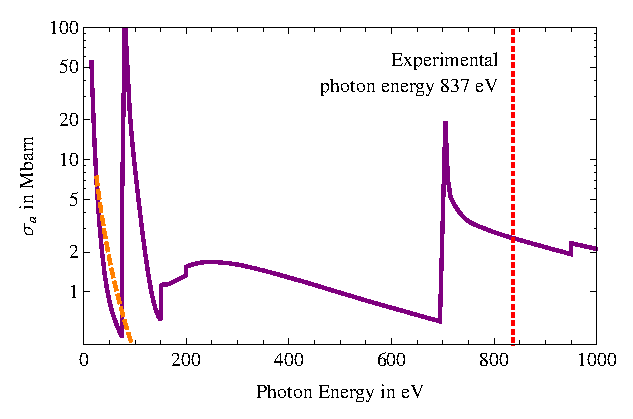
\includegraphics[width=0.80\textwidth]{images/photoionization.eps}
	\caption[Total absorption cross-sections for helium and xenon.]{Total absorption cross-sections $\sigma_{a}$ in megabarn for xenon (purple line) and helium (orange dashed). The photon energy of the described experiment is $\sim 837$ eV (red dashed). Data points from \citep{Elettra-2016-Website,Yeh-1985-AtmDat,Yeh-1993-GBSP}.}
	\label{fig:photoionization}
\end{figure}
 Imagine an electro-magnetic wave propagating in a medium with the above considerations. The wave travels along the $z$-axis and can be written as \citep{Als-Nielson-2011-JWS,Attwood-2007-CUP}
\begin{equation}
e^{i n k z}= \underbrace{e^{i \left(1-\delta\right)k z}}_{\text{phase shift}}\underbrace{e^{-\beta z}}_{absorption},
\label{eq:wave-in-medium}
\end{equation}
where $n$ is the complex refractive index, $\delta$ the real dispersion correction\index{dispersion correction!complex} resulting in a phase shift of the wave and $\beta$ being the imaginary dispersion correction resulting in a decline in amplitude of the wave\footnote{We jump between the wave and particle picture as it pleases us. Here, a decline in amplitude in the wave picture can be read as absorption in the particle picture.}. The relation between the complex refractive index $n$, $\beta$, and $\delta$ is explicitly given by
\begin{equation}
n=\frac{c}{v_{\text{phase}}}=1-\delta+i\beta.
\label{eq:complex-refractive-index}
\end{equation}
Let us now consider the atomic scattering factor. One would imagine that the acceleration of a bound electron in an atom is affected. Electrons that are tightly bound, e.g., in the K-shell, are less ``free'' than those with little binding energy. Overall, the atomic scattering factor must be reduced by a wavelength dependent amount, which we denote as $f^{'}$. The other wavelength dependent effect is absorption, which we can introduce as $f^{''}$. These two effects are called dispersion corrections to the atomic scattering factor, $f^{0}$. Let us include these corrections to the atomic scattering factor and note
\begin{equation}
f\left(\vec{Q=0},\hbar\omega\right)=f^{0}\left(Q=0\right)+f'\left(\hbar\omega\right)+i f''\left(\hbar\omega\right).
\label{eq:scattering-factor-dispersion-corr}
\end{equation}
In the limit of high photon energies $\hbar \omega$, bound electrons can be largely seen as free, as the binding energies become a minor factor, therefore $f'\left(\hbar\omega\right)\rightarrow 0$ and $f''\left(\hbar\omega\right)\rightarrow 0$. As the photon energies, $\hbar \omega$, are closer to the atomic level, which is the case at soft X-rays for many materials, $f'\left(\hbar\omega\right)$ and $f''\left(\hbar\omega\right)$ can become large factors.\\[1\baselineskip]
We can compare Equation \eqref{eq:complex-refractive-index} to Equation \eqref{eq:scattering-factor-dispersion-corr} and realize that we are allowed to define the dispersion relation through the atomic form factor as \citep[see][p.~76]{Als-Nielson-2011-JWS}
\begin{equation}
n= 1- \frac{2\pi \rho_{atom}r_{0}}{k^{2}}\left(f^{0}\left(\vec{Q}=0\right)+f'\left(\hbar\omega\right)+i f''\left(\hbar\omega\right)\right),
\label{eq:eq:complex-refractive-index-atomic-factors}
\end{equation}
with the atomic number density $\rho_{atom}$ and we identify explicitly
\begin{align}
\delta &= \frac{2 \pi \rho_{atom} r_{0}}{k^{2}}\left(f^{0}\left(\vec{Q}=0\right)+f'\left(\hbar\omega\right)\right),\quad \text{and}\\
\beta &= - \left(\frac{2\pi \rho_{atom}r_{0}}{k^{2}}\right)f''\left(\hbar\omega\right).
\label{eq:delta-and-beta}
\end{align}
We have already established in Equation \eqref{eq:wave-in-medium} that $\beta$ reduces the amplitude of the incoming wave through absorption. Using this insight about absorption, we can rewrite Equation \eqref{eq:delta-and-beta} and define $f''\left(\hbar\omega\right)$ in terms of being proportional to an absorption cross section, $\sigma_{a}$, which reads
\begin{equation}
f''\left(\hbar\omega\right)=-\left(\frac{k}{4\pi r_{0}}\right)\sigma_{a}.
\label{eq:f-2-definition}
\end{equation}
Figure \ref{fig:photoionization} shows the total absorption cross-sections $\sigma_{a}$ for xenon and helium at various photon energies. The photon energy of the experiment was $\SI{837}{\electronvolt}$. For helium, the photon energy is much greater than the binding energy and thus the absorption cross-section is low. For the thightly bound electrons in xenon, the absorption cross-section is relevant as the photon energy is near the atomic levels. The absorption cross-section shows a resonant-type behavior, when the photon energy would be directly on an atomic level. To get a better understanding of the absorption cross-section with regard to atomic levels, Table \ref{tab:xenon-photoionization-cross-section} and \ref{tab:helium-xenon-ionization} show the differential photo-absorption cross sections and ionization potentials for various energy levels and ionization configurations at the experimental photon energy $\SI{837}{\electronvolt}$ for xenon and helium. The calculations were performed with the Los Alamos Atomic Physics code based on \citep{Cowan-1981-Cal}.
\begin{table}
	\centering
		\begin{tabular}{ | c | c | c | c | }
			\hline
			Shell & Subshell & Cross-section & subshell ionization \\
				&	& in Mb & potential in eV \\ \hline
			K & 1s & - & 34630.0 \\ \hline
			L & 2s & - & 5466.4  \\ 
			\ & 2p & - & 4899.1 \\ \hline
			M & 3s & - & 1153.3  \\ 
			\ & 3p & - & 965.4 \\ 
			\ & 3d & 2.2505 & 682.7 \\ \hline
			N & 4s & 0.0305 & 223.7 \\ 
			\ & 4p & 0.1247 & 161.8 \\ 
			\ & 4d & 0.2587 & 68.2  \\ \hline
			O & 5s & 0.0040 & 27.3  \\ 
			\ & 5p & 0.0120 & 12.5  \\ \hline
		\end{tabular}
	\caption[Differential absorption cross-sections and ionization potentials for xenon.]{Differential absorption cross-sections and ionization potentials for certain electronic configurations of xenon at 837eV. Calculations based on \citep{Cowan-1981-Cal}.}
	\label{tab:xenon-photoionization-cross-section}
\end{table}
It appears that certain energy levels, or here subshells if one disregards the hyperfine structure\footnote{A shift in energy levels due to interaction of electrons with the nucleus \citep[see][p~166~ff.]{Demtroder-2005-Springer}.}, tend to have a higher absorption cross-section than others. This brings us back to the picture of the forced harmonic oscillator, where an electron is driven by a light field. If the frequency of the light field is close to the eigenfrequency of the bound electron, in other words, if the energy of a photon is close to the energy level of a bound electron, the system is in resonance and absorption is highly likely. As the photon energy and electron level energy differ, the system is off resonance and it is less likely to absorb a photon. As energy levels in atoms are discrete, electrons can only be excited from one energy level to another or need a certain (minimal) ionization energy\index{ionization!energy} to ionize an atom and excite an electron into the continuum. Therefore, the likelihood of a core-electron that is strongly bound being ionized is by far the most probable using X-rays.
\begin{table}
	\centering
		\begin{tabular}{ | c | c | c | c | }
		\hline
%			Configuration & ionized subshell & Cross-section (Mbarn) & Helium ionization potential in eV \\ \hline
			El. Configuration, & Ionization & Cross-section  & subshell ionization  \\
			and ionized subshell & of subshell & $\sigma_{a}$ in Mbarn & potential in eV \\ \hline
			He\textsuperscript{+0},\ 1s2 & 1s2 & 0.0007 & 24.4 \\ \hline
			He\textsuperscript{+1},\ 1s1 & 1s1 & 0.0005 & 54.4 \\ \hline
			Xe\textsuperscript{+0},\ 5p6 & 3d10 & 2.2505 & 682.7 \\ \hline
			Xe\textsuperscript{+1},\ 3d9 & 3d9 & 2.1487 & 733.6 \\ \hline
			Xe\textsuperscript{+1},\ 5p5 & 3d10 & 2.2443 & 693.7 \\ \hline
			Xe\textsuperscript{+2},\ 5p4 & 3d10 & 2.2390 & 705.9 \\ \hline
		\end{tabular}
	\caption[Absorption cross-sections and ionization potentials for xenon and helium]{Absorption cross-sections $\sigma_{a}$ and ionization potentials for certain electronic configurations, including certain ionization profiles. Calculations based on \citep{Cowan-1981-Cal}.}
	\label{tab:helium-xenon-ionization}
\end{table}
When a core electron gets ionized, the electronic structure changes and particular ionization energies and (absorption) cross-sections change. To discuss the parameters that are most applicable to this thesis, a comparison of the most probable transition at the photon energy 837eV is given for helium and xenon in Table \ref{tab:helium-xenon-ionization}. The ionization energies change drastically, whether a core electron or a less tightly bound electron is ionized. As per absorption cross-sections, helium can be considered transparent and xenon atoms have a much larger absorption cross-section. The number of ionization configurations can become rather complex and the table shall give the reader merely a broad understanding of some likely configurations.\\[1\baselineskip]
%Similarly to the estimate made in Equation \eqref{eq:absorption-cross-section}, it is very unlikely for an atom to absorb more than two photons in one pulse of a free electron laser, which is why we only consider the most probably transitions here to get an understanding how the absorption cross-sections change.\\
% \begin{table}
% 	\centering
% 		\begin{tabular}{ | c | c | c | c | }
% 		\hline
% 			El. Configuration, & Ionization & Cross-section  & subshell ionization  \\
% 			and ionized subshell & of subshell & $\sigma_{a}$ in Mbarn & potential in eV \\ \hline
% 			Xe\textsuperscript{+0},\ 5p6 & 3d10 & 2.2505 & 682.7 \\ \hline
% 			Xe\textsuperscript{+1},\ 3d9 & 3d9 & 2.1487 & 733.6 \\ \hline
% 			Xe\textsuperscript{+1},\ 5p5 & 3d10 & 2.2443 & 693.7 \\ \hline
% 			Xe\textsuperscript{+2},\ 5p4 & 3d10 & 2.2390 & 705.9 \\ \hline
% 		\end{tabular}
% 	\caption{caption. Calculations based on \citep{Cowan-1981-Cal}.}
% 	\label{tab:xenon-ionization}
% \end{table}{}
The total atomic scattering factors, $f^{0}$, for neutral and ionized, helium and xenon can be found in Table \ref{tab:helium-xenon-el-scattering-crossection}. It is interesting to see that although a xenon atom has only 27 times more electrons than a helium atom the scattering factor $f^{0}$ of neutral xenon is over 900 times stronger than helium. Upon ionization, the absolute changes in $f^{0}$ of helium are therefore smaller compared to xenon. The relative change in helium of $f^{0}$ after one electron is ionized is $\sim 75$ \%, thus (ionized) helium barely scatters. As xenon has multiple occupied subshells, the scattering factors of different ionized subshells are shown in Table \ref{tab:helium-xenon-el-scattering-crossection}. As discussed, it is most likely to ionize the xenon 3d subshell, however, within a few femtoseconds subsequent relaxation processes\footnote{See the following Section \ref{sec:relaxation}.} lead to different ionization configurations, for example a double ionized 5p subshell. For the scattering factor, there is little change whether the 3d or 5p subshell becomes ionized and the change in $f^{0}$ is only $\sim 0.05$\%. As xenon has 54 electrons, the relative change upon ionization of one electron in $f^{0}$ is only 3 \%. Xenon is therefore a much stronger scatterer than helium and xenon still scatters well upon ionization of inner or outer shell electrons.  
\begin{table}
	\centering
		\begin{tabular}{ | c | c | }
		\hline
			El. Configuration, & Scattering factor \\
			and ionized subshell & $f^{0}$ in barn \\ \hline
			He\textsuperscript{+0},\ 1s2 & 2.5539  \\ \hline
			He\textsuperscript{+1},\ 1s1 & 0.649465  \\ \hline
			Xe\textsuperscript{+0},\ 5p6 & 1874.36  \\ \hline
			Xe\textsuperscript{+1},\ 3d9 & 1813.56  \\ \hline
			Xe\textsuperscript{+1},\ 5p5 & 1814.68  \\ \hline
			Xe\textsuperscript{+2},\ 5p4 & 1754.08  \\ \hline
		\end{tabular}
	\caption[Atomic scattering factors for helium and xenon.]{Atomic scattering factor $f^{0}$ for certain electron configurations. Calculations based on Equation \eqref{eq:scattering-integral}. From \cite{Ho-2016-PC}.}
	\label{tab:helium-xenon-el-scattering-crossection}
\end{table}
In the experiment described in the following chapters, the photon energy is explicitly chosen to have a comparably high absorption cross-section for xenon -- but is off the absorption resonance --, a comparably low absorption cross-section for helium, and a wavelength short enough to receive high resolution images through coherent diffraction imaging. In such a setting, xenon is most likely to absorb X-rays and helium can be considered transparent.
%
%
%
%
%
\subsection{Charge migration}\label{sec:relaxation}
%%%
\begin{figure}
	\centering
		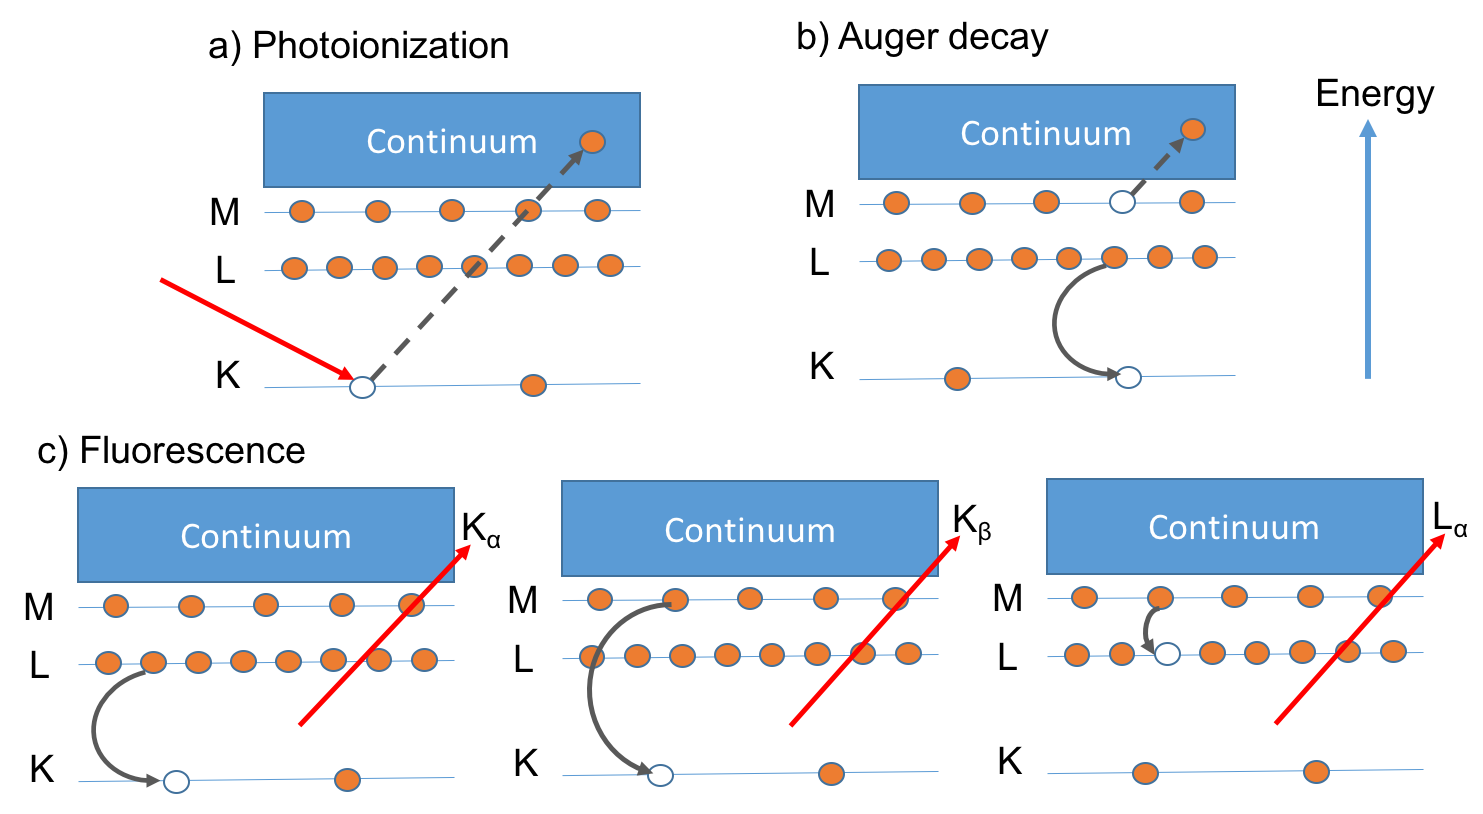
\includegraphics[width=0.80\textwidth]{images/el-relaxation.png}
	\caption[Schematic illustration of common charge transfer processes]{Schematic illustration of common charge transfer processes. a) Photoionization: Describes a direct emission of a K-shell electron after absorbing an X-ray photon. b) Auger decay: A relaxation process, where a K-shell hole is filled with an electron from the L-shell and the remaining energy is released through emission of an electron in an outer shell. c) Fluoresence:An electron hole is filled with an electron from an outer shell and the remaining energy is released through photons. After \citep[][p.~19]{Als-Nielson-2011-JWS}.}
	\label{fig:el-relaxation}
\end{figure}
After an atom has been (core-)ionized due to absorption of a photon as depicted in Figure \ref{fig:el-relaxation}a, the atom is usually not in its most energetically favorable state. In order to emit energy and transition into its new ground state, the atom can emit particles according to the schematics in Figure \ref{fig:el-relaxation}b-c. In a fluoresence decay (\ref{fig:el-relaxation}c), the electron hole in the (K-)shell is filled by an electron in an energetically higher shell, here L or M shell, and thereby emits a photon of the discrete energy difference between the transitioning levels. If one spectrally resolves the signal, the discrete peaks are element-specific and modern photoemission spectroscopy can yield insight into, for example, element identification, excitation dynamics or chemical bonding.
\begin{figure}
	\centering
		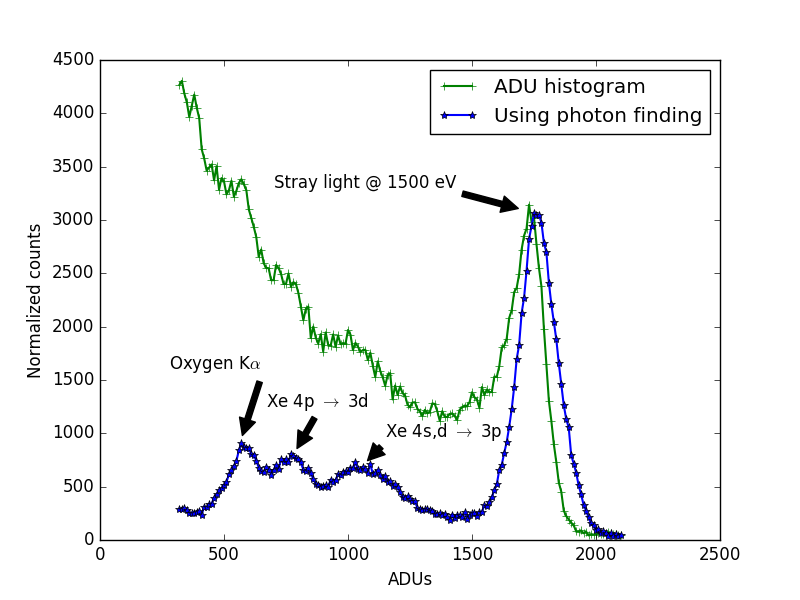
\includegraphics[width=.49\textwidth]{images/pnCCD-histogram.png}
		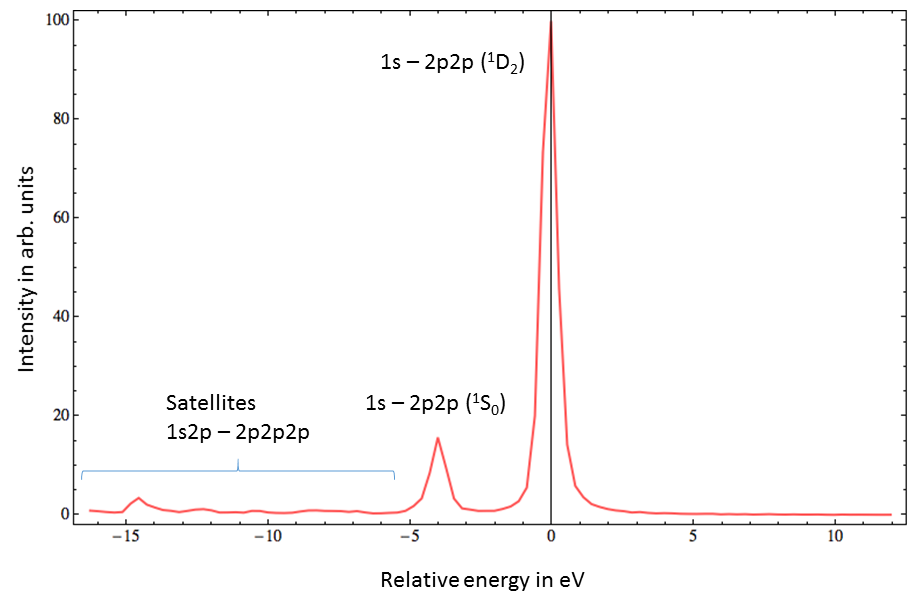
\includegraphics[width=.49\textwidth]{images/auger-spectra.png}
	\caption[Fluorescence spectra from xenon and neon K-LL Auger spectrum.]{Left spectra shows fluorescence peaks from xenon and oxygen illuminated with 1.5keV photons from the LCLS; detected with pnCCD detectors \citep{Bucher-2016-Unpublished, Rudek-2012-NatPho}. The green curve is an ADU histogram of the pnCCD detector and the blue curve uses a coalescent photon finder. Right, partial K-LL Auger spectrum with rel. energy 0 corresponding to 804.5 eV. Spectrum measured with photoelectron spectrometer \cite{Bucher-2014-Unpublished}, peaks identified as in \citep{Krause-1970-PhysLettA}.}
	\label{fig:pnCCD-histogram}
\end{figure}
The left panel of Figure \ref{fig:pnCCD-histogram} shows measured fluorescence lines of oxygen and xenon. In this measurement, xenon atoms and residual oxygen atoms have been illuminated with 1500 eV photons from the Linac Coherent Light Source and the fluorescence photons have been measured with the LAMP pnCCD detectors that are described in Section \ref{sec:pnCCD}. The green curve is a ADU histogram of the pixel-detector using the detector calibrations described in Section \ref{sec:pnccd-corr}. The blue curve additionally uses a photon-finding algorithm as the signal from just one fluorescence photon splits into multiple pixels. The coalescent-photon finding algorithm\index{algorithm!coalescent-photon finding} looks for pixels above a certain threshold and includes neighboring pixels above a certain, lower threshold, thus correcting the measured signal to yield a proper ADU count per photon.\\[1\baselineskip]
%
The Auger decay is another possibility for the atom to emit energy through a two-step process. One, an outer shell electron is emitted into the continuum, the so-called \textit{Auger-electron}\footnote{Named after the French physicist Pierre Auger.}. Two, another electron in the atom simultaneously fills the electron-hole. An \textit{Auger decay} occurs typically on the few femtosecond timescale after ionization \citep{Krause-1970-PhysLettA}. Emitted Auger-electrons have discrete energies depending on the combination of electrons involved in the process. Similar to fluorescence spectroscopy, one can use this attribute to, for example, identify elements or calibrate energies. Figure \ref{fig:pnCCD-histogram} right shows a partial K-LL\footnote{This nomenclature means a single hole in the K-shell is followed by a two holes in the L shell after the Auger decay.} Auger spectrum from neon illuminated by 1050 eV photons from the LCLS and measured with a hemispherical analyzer as described in \citep{Bucher-2014-Unpublished}. In this example, neon is ionized in the K-shell and an electron-hole in the 1s shell is created. An electron from the L-shell fills the 1s hole and another electron from the L-shell, the Auger electron, is emitted into the continuum. As there is a variety of electronic configurations that can be involved in this process multiple peaks appear for similar occupation configurations, e.g., 1s - 2p2p. More complex structures, called satellites, appear when the atom is already ionized, for example, the atom has a hole in the L-shell and then an absorption that creates another hole in the K-shell. This will lead to KL-LLL satellites.\\
Similar to the Auger decay, where electrons from an outer shell are involved in the relaxation process, the transition can also be of the same shell and is then called a Coster-Kronig transition. Relevant transitions are for example the N-NN Coster-Kronig transitions in xenon \citep{Coster-1935-Physica}.
%\\So far we have looked at X-ray induced processes from atoms. Extended objects, whether a bio-molecule or a cluster, will respond differently than just the atoms they consist of. Nanometer-sized objects will develop a distinct character due to their electronic bond with other particles. This includes rare-gas clusters that are weakly bound Van der Waals forces. We shall explore this behavior in the next Section \ref{sec:ionizatin-of-ext-obj}.
%
%
%
%
\section{Ionization of clusters in intense X-ray pulses}\label{sec:ionizatin-of-ext-obj}
%%%%%%%%%%%%%%%%%%%
%- Short introduction coming from inelastic scattering
%%%%%%%%%%%%%%%%%%%
The response of a cluster upon irradiation with light often differs from just the atomic response. Collective effects change the (microscopic) sample environment and it is now the collective of atoms that generate a response to the interacting light. Clusters provide, therefore, a testbed environment to study collective effects ranging from atomic, to molecular and to bulk material attributes. While we went over some benefits of using clusters in Section \ref{sec:cluster-theory}, it shall also be said that they provide an ideal testbed sample to control light-driven many-particle processes \citep{Fennel-2010-RMP}. In this section, we study how rare-gas clusters respond to femtosecond long, high intense X-ray pulses and reflect on recent experiments.
%
%
%
\subsection{Formation and expansion of a nanoplasma}\label{sec:nanoplasma-expansion}
%%%%%%%%%%%%%%%%%%%%%%%%
%- Step by step explanation on the formation of a nanoplasma
%%%%%%%%%%%%%%%%%%%%%%%%
\begin{figure}
	\centering
		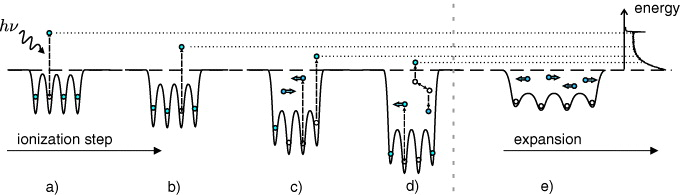
\includegraphics[width=1.00\textwidth]{images/nano-plasma-schematic.jpg}
	\caption[Schematic of the nanoplasma creation and expansion.]{Schematic of the nanoplasma creation and expansion. In step a) X-ray photons ionize electrons from a cluster. b) Subsequent \textit{multistep ionizations}\index{ionization!multistep} try to relax the electronically excited system, deepening the Coulomb potential of the cluster. Step c) shows a deepened Coulomb potential of the cluster, due to which the multistep ionization becomes (partially) frustrated and electrons are trapped in the potential. In step d) trapped electrons collide and start to thermalize. Collisions can lead to emission of trapped electrons. d) The superheated nanoplasma starts to expand. From \citep[\href{https://creativecommons.org/licenses/by/3.0/}{\ccby}]{Arbeiter-2011-NJP}.}
	\label{fig:nano-plasma-schematic}
\end{figure}
 Let us recapture the scattering and absorption effects discussed in last section Section \ref{sec:light-matter-interaction}. Equation \eqref{eq:scattered-amplitude} indicates how the diffracted amplitude of a nanoparticle can be calculated. Although we disregard inelastic or incoherent processes, the modulo of the amplitude is close to actual measured scattering patterns. However, if we consider the resonant effects discussed in Section \ref{sec:absorption}, it should be clear that the structure factor of a nanoparticle is affected by the dispersion corrections $f'\left(\omega\right)$ and $f''\left(\omega\right)$ that reduce the atomic scattering length, $-r_{0}f^{0}\left(\vec{Q}\right)$. On the one hand, a dominating change in the atomic scattering length is driven by the absorption process that we introduced via the imaginary dispersion correction $i f''\left(\omega\right)$. Upon ionization, the atomic scattering factors, $f^{0}\left(\vec{Q}\right)$, change as the absorption cross-sections start to vary. These small changes are indicated in Table \ref{tab:helium-xenon-ionization} and such processes are exptected to occur on the few femtoseconds timescale, on which the ionization dynamics occur. Additionally, due to photoionized electronsin the atom, the atomic scattering factors change on the few femtoseconds timescale. Such small changes are indicated in Table \ref{tab:helium-xenon-el-scattering-crossection}. On the other hand, there are X-ray induced effects that change the scattering behavior of the collective of atoms, i.e., the cluster. We know from previous experiments \citep{Gorkhover-2016-NatPho} that these changes are related to the nanoplasma expansion and can significantly affect diffraction patterns.\\[1\baselineskip]
%
 Let us follow Figure \ref{fig:nano-plasma-schematic} and \citep{Arbeiter-2011-NJP,Bostedt-2010-JPB} in the next five steps to get a better understanding of the nanoplasma phase-transition. Step a) of the nanoplasma transition\index{nanoplasma!transition}, the cluster gets ionized due to intense radiation\footnote{The wavelength of radiation must be above the ionization threshold of at least one subshell, however, it must not be X-rays with a wavelength on the nanometer length scale.}. Step b), further ionization through emission of photo electrons and Auger electrons lead to a so-called \textit{multistep ionization}\index{ionization!multistep} that steepens the Coulomb potential\index{Coulomb potential} \citep{Wabnitz-2002-Nature,Laarmann-2004-PRL,Bostedt-2008-PRL}. Step c), the multistep ionization is suppressed (or frustrated) because the Coulomb potential depth is larger than the atomic excess energy of photo- and Auger electrons. The emitted electrons are now trapped in the cluster potential and are \textit{quasi-free}. Upon increasing \textit{inner ionization}\index{ionization!inner}, the nanometer-sized object undergoes a phase transition to a nanoplasma\footnote{Plasma is another state of matter, similar to solid, liquid and gaseous, where molecular bonds dissociate and positive and negative particles are present in increasing numbers.}. Step d), the temperature of the nanoplasma is initially defined by the atomic excess energies (a rather discrete spectrum) but collisions with other particles lead to a (kinetic) energy distribution of the electrons that is similar to thermal distributions and can be measured via the spectra of evaporated electrons \citep{Laarmann-2005-PRL,Bostedt-2010-NJP}. Step e) Hydrodynamic and Coulomb forces drive an expansion of the cluster and the cluster will ultimately disintegrate. The hydrodynamic portion of the force is due to the developing hot plasma and the resulting increase in outward pressure, whereas the Coulomb portion comes from the repelling force of like charges. Both forces reasonably describe the expansion process, are not mutually exclusive and depend mostly on sample size and irradiation technique.\\[1\baselineskip]
 %
Regarding the sample size, large clusters efficiently trap electrons in their Coulomb potentials such that the quasi-free electrons thermalize and subsequently heat the nucleus. The hot nanoplasma system then tries to expand due to the increase in internal pressure. Electrons thermalize on the attosecond timescale and simulations show that the energy transfer to the ions can be as fast as 50 fs \citep{Arbeiter-2010-PRA}. Small clusters trap photo- and Auger-electrons less efficiently and electrons are free such that the heating process is suppressed. In the case of small clusters, the ions see the repelling force due to Coulomb interaction of like charges with each other \citep{Lezius-1998-PRL}.\\[1\baselineskip]
%
The nanoplasma expansion is also wavelength dependent. At optical to UV wavelengths strong field ionization can lead to ionization of clusters and a subsequent nanoplasma expansion \citep{Springate-2000-PRA}. At VUV, XUV and soft X-rays, direct photoionization becomes the main driver of the nanoplasma expansion and depending on the wavelength, certain multistep ionization cascades are enabled \citep{Arbeiter-2011-NJP}. It remains to discuss the radiation intensity, which affects the ultimately achieved charge-state combination. The more intense the radiation is, the more energy is absorbed by the cluster. For the nanoplasma this determines the electron temperature and possibly the expansion speed.
%Following a similar line of argumentation, low energy ionizing photons allow efficient trapping of photo and Auger electrons, thus favorable conditions for a hydrodynamic expansion. Conversely, high photon energies\footnote{Meaning hard X-ray with wavelenghs on the {\AA}ngstrom length scale as soft X-rays have similar photon energies as trapping potentials and multistep ionization deepens the Coulomb potential enough.} lead to more atomic excess energy such that more electrons overcome the trapping potential, thus favorable conditions for a Coulomb expansion. However, this line is very element dependent and atoms with large atomic mass, such as Xenon\footnote{Find ionization energies for specific subshells in Table \ref{tab:xenon-photoionization-cross-section} and deepened Coulomb potential ionization energies after ionization of Xe, here Xe$^+1$ and Xe$^{+2}$ for different subshell ionization configurations, in Table \ref{tab:helium-xenon-ionization}.} would require photon energies $E_{ph}$ of $5.5keV\ll E_{ph} < 34.6k eV$ or $34.6keV\gg E_{ph}$ and since mostly the immediate process upon photon absorption is wavelength dependent and the electron trapping of the majority of subsequent multistep ionizations will be mostly dependent on the cluster size.\\
%
%
%
\subsection{Imaging of transient states}
\begin{figure}
	\centering
		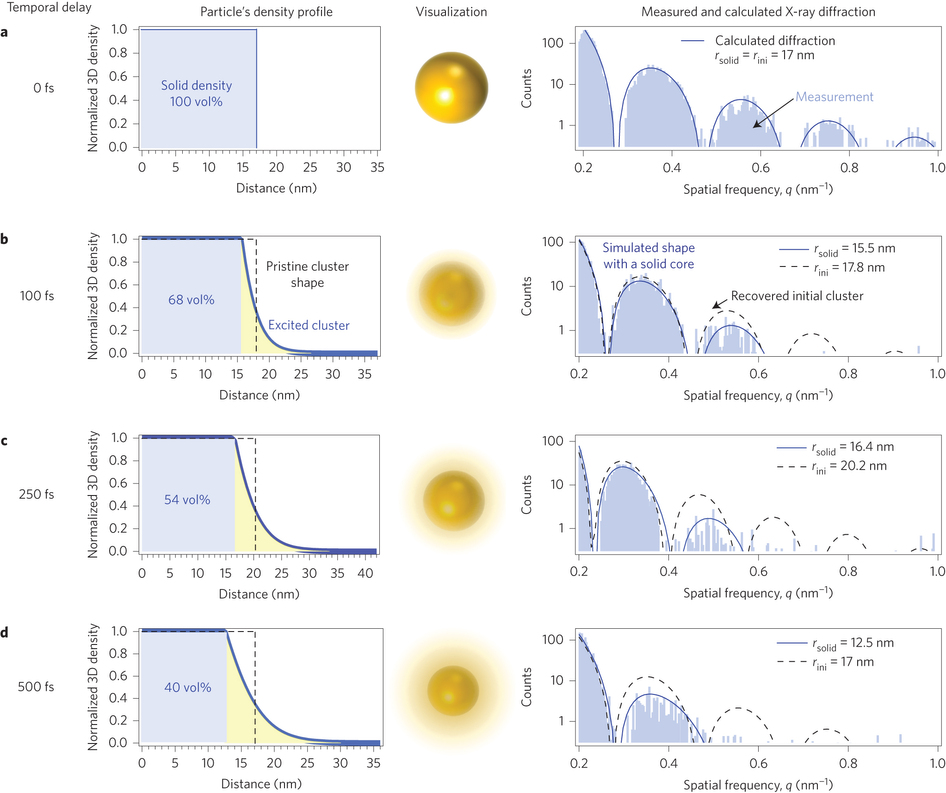
\includegraphics[width=1.00\textwidth]{images/tais-nat-photonics.jpg}
	\caption[Measurement and simulation of the nanoplasma expansion in Xe-clusters.]{Xe-clusters after being pumped with a NIR laser pulse and probed at a certain time delay (indicated left) with a LCLS pulse. Left series, simulation of electron densities. Right series, measured diffraction patterns. The diffraction patterns show a decrease in intensity at larger q values, when the delay is increased. This can be explained through expanding electron densities, i.e., a nanoplasma expansion. Fourier transformation of electron densities are fitted to the measurement for a solid sphere (dashed line) and an expanding sphere (solid line). From \citep{Gorkhover-2016-NatPho}. Reprinted with permission from Nature Publishing Group.}
	\label{fig:tais-nat-photonics}
\end{figure}
%The nanoplasma transition is so interesting is because every matter irradiated by a free-electron laser will undergo a nanoplasma transition and finally disintegrate. This is a challenge for structural biology and called radiation damage  or sample damage \citep{Neutze-2000-Nature}. Sample damage changes the structure of a biomolecule and it is particularly the structure many scientists want to investigate. In order to prevent falsified measurements, one needs to understand the nanoplasma transition as it occurs while the pulse is propagating through the sample.
To study the nanoplasma transition, a coincident imaging and spectroscopy technique has proven successful \citep{Bostedt-2012-PRL}. First experiments aimed to reveal correlations between the diffraction patterns and the ion spectroscopic data \citep{Gorkhover-2012-PRL,Rupp-2016-PRL}. The advent of pump--probe techniques has been combined with the coincident measuring technique and recently, snapshots were taken of the expanding electron density \citep{Gorkhover-2016-NatPho}. The snapshots are shown in Figure \ref{fig:tais-nat-photonics}. In this particular study, an infra-red laser (pump) was used to cause a nanoplasma transition in a xenon cluster and subsequently image this state with an XFEL pulse (probe). As the time delay between pump- and probe-pulse is varied, the resulting diffraction patterns of the 15-20 nm Xe-cluster show declining intensities at larger scattering angles with increasing time delay, $\Delta t>100$ fs. The loss in signal could be explained through an expanding electron density\index{electron density!expanding} \citep{Hau-Riege-2008-PRE,Peltz-2014-PRL}. The electron density expands increasingly over time due to the Coulomb and Hydrodynamic forces. First, the outer layers expand, and second, for larger time delay also the inner atomic layers start to expand. In that study, an electron temperature of $\sim 200$ eV could be measured by comparing plasma simulations to the ion spectroscopy signal. The spatial resolution of the diffraction patterns has been estimated to be 8 nm, but by assuming a spherical shape of the clusters, the electron density model is sensitive below this resolution.\\[1\baselineskip]
\begin{figure}
	\centering
		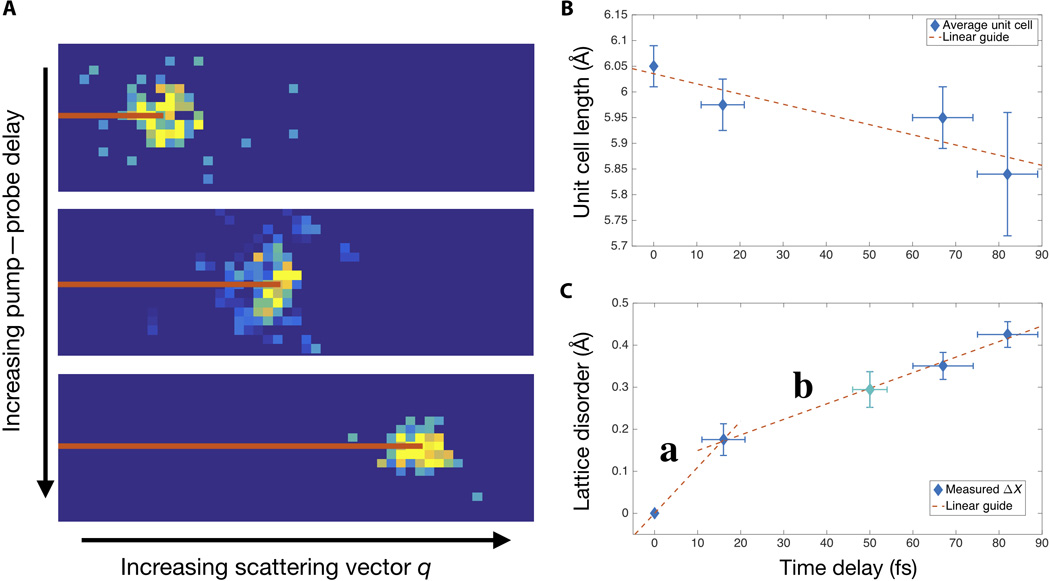
\includegraphics[width=0.80\textwidth]{images/ken-science.jpg}
	\caption[Experiment that shows early evolution of the nanoplasma transition.]{X-ray pump--X-ray probe scattering experiment on an Xe-cluster that shows an early evolution of the nanoplasma transition. A, single-shot Bragg peaks at varying time delays. The scattering vector q increases over time delay. B, unit cell length over time delay. The unit cell length decreases, therefore the cluster shrinks in size. C, Lattice disorder over time delay. The measured fcc lattice is becoming disordered after being pumped with an X-ray pulse. From \citep{Ferguson-2016-SciAdv}. Reprinted with permission from AAAS.}
	\label{fig:ken-science}
\end{figure}
In another study with shorter time delays of $\Delta t<100$ fs, xenon clusters compress in size \citep{Ferguson-2016-SciAdv}. Since clusters form as a crystal\footnote{See Section \ref{sec:homogenous-cluster}.}, one can determine their structure through crystallographic approaches as it is explained in full detail in \citep[][chapter 5]{Als-Nielson-2011-JWS}\footnote{In short, crystals scatter light and create Bragg spots at large $\vec{Q}$-values. These Bragg spotts occur when Bragg's law is fulfilled. Bragg's law reads $m \lambda = 2d \sin\left(\frac{\Theta}{2}\right)$,\index{Bragg's law} with $m$ being an integer, $\lambda$ being the wavelength of the scattered light, $d$ the distance between crystalline layers and $\Theta$ the scattering angle. When Bragg's condition is fulfilled, the rays interfere constructively and the location of the Bragg peaks gives insight to the crystalline structure.}. Figure \ref{fig:ken-science}a shows Bragg peaks, which occur under certain conditions over the scattering vector, $\vec{Q_{\text{peak}}}$. In the figure, the signal moves to larger scattering vectors and, as $\vec{Q_{\text{peak}}}=\frac{2\pi}{a}$, the unit cell length $a$ shrinks over the time delay $\Delta t =$ \SIrange{0}{100}{\femto\second}. This unintuitive and contradictory result is attributed to the changes in electronic configuration upon ionization. Electrons that are trapped in the cluster's Coulomb potential have an increased mobility and are able to contribute comparably to valence electrons and, therefore, change the chemical bonding character of the Van der Waals cluster. As a result, the unit cell changes on the {\AA}ngstrom length scale and the lattice becomes increasingly disordered (see Figure \ref{fig:ken-science}c).\\[1\baselineskip]
These two studies allow us to conclude that the nanoplasma transition is a multistep process. First, the initial ionization occurs, followed by an increased Coulomb potential that traps electrons, which then change the structure of the nanosample, e.g., compression of a lattice. Eventually, the system becomes strongly ionized and hot such that Coulomb and hydrodynamic forces start an expansion of the system until the sample disintegrates into its atomic components.
%
%
%
\subsection{Tampered layers to inhibit the nanoplasma expansion}
%%%%%%%%%%%%%%
%- Step by step explanation on the formation of the nanoplasma, pointing out the differences between tampered and pristine clusters
%
%
%%%%%%%%%%%%
%To overcome radiation damage, the most common method is to \textit{outrun} radiation damage\index{radiation damage} processes using very short pulses \citep{Neutze-2000-Nature}.
As we have discussed, the nanoplasma phase-transition occurs on the femtosecond timescale and affects diffraction patterns. To \textit{outrun} this radiation damage, pulses from the XFEL must be shorter than the lifetime of Auger processes, thus a few femtoseconds long. And by limiting the XFEL pulse duration, one limits the pulse energy\index{pulse energy} as current bunch compression methods typically generate much less fluence. Often, this fluence is not enough and means that many coherent diffractive imaging experiments are currently performed with pulse widths of 40 fs or more to generate enough scattered intensity. But even if these technical limitations can be overcome, outrunning radiation damage does not circumvent photoionization and it is therefore expected that few-femtoseconds long pulses have spatial resolution limitations \citep{Aquila-2015-StrucDyn}. To be more precise, it is an open question, whether electron densities and particular bonding configuration are obtainable by solely outrunning radiation damage. Although radiation damage is unavoidable it can be mitigated in several ways. One way to mitigate radiation damage is to simulate the effects, however, this can only be done for small particles. Another way is to fundamentally increase resolution in single particle imaging due to prior alignment of particles such that their orientation is known while the image is taken. Molecule alignment has seen some success for small molecules \citep{Kupper-2014-PRL}, but it is currently unknown, whether this is applicable for larger molecules. The strong light fields that are needed to align the molecules, may change their structure. Here, it should be noted that recent advances with diffractive imaging algorithms made it possible to computationally determine the orientation of a particle at the time of imaging \citep{Loh-2009-PRE,Ekeberg-2015-PRL}. The orientation can be atomatically determined -- without prior knowledge -- when at least a few hundred diffraction images are provided. However, in this thesis, we shall discuss a method to reduce the effects of radiation damage through artificial tamper layers. Artificial shells around a sample supply it with electrons and function as a sacrificial layer that protects the sample \citep{Hau-Riege-2010-PRL}. For aerosol particles, this method has only been investigated through ion spectroscopy \citep{Hoener-2008-JPB,Ziemkewitz-2017-unpublished}.\\[1\baselineskip]
\begin{figure}
	\centering
		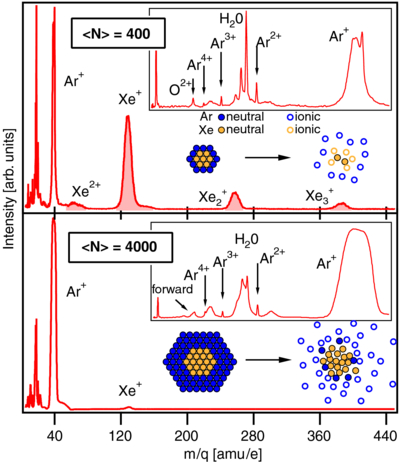
\includegraphics[height=0.50\textwidth]{images/Hoener-image.jpg}
	\caption[Time of flight spectra of argon and xenon core-shell systems.]{Time of flight (TOF) traces of argon and xenon core shell systems irradiated with 93eV X-ray pulses from FLASH\index{Free electron LASer in Hamburg!FLASH}. At this energy, mostly Xe is ionized and the ionized atoms create a steep Coulomb potential that traps electrons towards the center of the cluster. The top panel shows smaller clusters with 400 particles, in which the trapping is inefficient, few electron-ion recombinations occur, thus Xe and Ar ions are detected in the TOF detector. The bottom panel shows large clusters with 4000 particles and a thicker argon shell. Here, Xe-ions recombine in the center and the TOF shows mostly Ar-ions as the neutral xenon remains undetected. From \citep[\href{https://creativecommons.org/licenses/by/3.0/}{\ccby}]{Hoener-2008-JPB}.}
	\label{fig:Hoener-image}
\end{figure}
In the study shown in Figure \ref{fig:Hoener-image}, a core-shell system of argon and xenon was constructed and here xenon is to the sample and argon corresponds to the sacrificial layer around the particle (see figure). The heterogeneous clusters were irradiated with 93 eV photons from \textit{FLASH}\footnote{Short for \textbf{F}ree electron \textbf{LAS}er in \textbf{H}amburg. An extreme ultra violet (XUV) free electron laser in Hamburg, Germany.}\index{Free electron LASer in Hamburg!FLASH}. At this photon energy, mostly xenon atoms are ionized. As described in the nanoplasma creation process (see Section \ref{sec:nanoplasma-expansion}), the increasingly ionized cluster creates a steep Coulomb potential, trapping electrons. Trapped electrons are available for recombination with the ionized atoms. In the small core-shell system of ArXe with 400 particles (Figure \ref{fig:Hoener-image} top-panel), the time of flight mass spectroscopy\index{time of flight!mass spectroscopy} data show Xe and Ar ions. These ions mean that the charge recombination is suppressed and the cluster disintegrates upon irradiation. In the large ArXe-cluster system with 4000 particles (bottom-panel), mostly Ar ions are in the TOF data. These ions mean that the Xe-ions in the center of the cluster recombine with the electrons that were attracted to the center of the core-shell system due to the steep Coulomb potential of the large cluster. Neutrally charged xenon is not detected by the TOF detector. The Ar-ions in the outer layers contributed electrons to the center of the cluster but were shed off the mixed ArXe-cluster. It is also evident that the argon atoms in the large cluster case release more kinetic energy than in the small cluster case, which is a size-dependent effect that shows an energy transfer process from the initially ionized Xe-core to the Ar-shell.
%
%
%
%